\documentclass[11pt,a4paper]{article}
\usepackage[utf8]{inputenc}
\usepackage[T1]{fontenc}
\usepackage{lmodern}
\usepackage[margin=2.1cm]{geometry}
\usepackage{amsmath,amssymb,amsthm,mathtools}
\usepackage{booktabs,array,multirow}
\usepackage{graphicx,float}
\usepackage{xcolor}
\usepackage{microtype}
\usepackage{xurl}
\usepackage[breaklinks=true,colorlinks=true,linkcolor=blue!60!black,citecolor=blue!60!black,urlcolor=blue!60!black]{hyperref}

\emergencystretch=3em
\allowdisplaybreaks
\let\origunderscore\_
\renewcommand{\_}{\origunderscore\penalty200\relax}

\graphicspath{{results_tortoise_v1_5/figures/}{results_tortoise_v1_4/figures/}{figures/}{./}}

\newtheorem{theorem}{Theorem}[section]
\newtheorem{proposition}[theorem]{Proposition}
\newtheorem{corollary}[theorem]{Corollary}
\theoremstyle{remark}
\newtheorem{remark}[theorem]{Remark}

\title{\textbf{The Toric Architecture of Extreme Animal Longevity and Biological Immortality:}\\
\large Exact Zero-RNG Klein $V_4$ Spectral Algebra, Archosaurian Stasis, and Five Evolutionary Genomic Strategies Across 30 Animal Species}

\author{%
\textbf{Victor Logvinovich}$^{1}$ and \textbf{Jean-Claude Perez}$^{2}$\\[6pt]
\small $^{1}$Master of Physical and Mathematical Sciences, Researcher in Pedagogical Sciences (Mathematics),\\
\small Kobrin, Belarus. \texttt{lomakez@icloud.com}, ORCID: \href{https://orcid.org/0009-0007-2040-6955}{0009-0007-2040-6955}\\[4pt]
\small $^{2}$PhD in Mathematics and Computer Science, Retired IBM AI European Research Centre, Montpellier;\\
\small Luc Montagnier Foundation. \texttt{jeanclaudeperez2@gmail.com}, ORCID: \href{https://orcid.org/0000-0001-6446-2042}{0000-0001-6446-2042}
}
\date{November 27, 2026 \quad (\textit{Audited Edition v1.6; Engine v1.5.0, 64/64 Zero-RNG Self-Tests})\\[4pt]
\small Repository: \href{https://github.com/Dr-Logvinovich/longevity-codon-torus}{\nolinkurl{github.com/Dr-Logvinovich/longevity-codon-torus}}\\
\small Engine: \href{https://github.com/Dr-Logvinovich/longevity-codon-torus/blob/main/tortoise_longevity_torus_v1_0.py}{\nolinkurl{tortoise_longevity_torus_v1_0.py}}}

\begin{document}
\maketitle

\begin{abstract}
Can macro-scale DNA architecture distinguish a 190-year-old giant tortoise, a 400-year-old Greenland shark, a 507-year-old ocean quahog, a 100-year-old negligibly senescent lobster, eusocial insect queens, and biologically immortal cnidarians from ephemeral animals without Monte Carlo sampling or fitted parameters?
Extending the exact Zero-RNG double-stranded codon-torus framework on $\mathbb{T}_4^3 = (\mathbb{Z}/4\mathbb{Z})^3$ to a 30-species animal kingdom atlas spanning nearly four orders of magnitude in lifespan---from $0.06\text{ yr}$ (\textit{Caenorhabditis elegans}) and $0.15\text{--}0.25\text{ yr}$ Diptera to $507\text{ yr}$ (\textit{Arctica islandica}) plus two biologically immortal cnidarians (\textit{Hydra vulgaris} T2T and \textit{Turritopsis dohrnii})---alongside 30 longevity orthologs across 12 vertebrates, we establish six empirical and algebraic laws (Theorems~L1--L8g), verified by 64/64 automated algebraic self-tests and intra-chromosome split-half reliability $\cos_{\mathrm{Beyond\text{-}M2}}(\mathrm{L},\mathrm{R}) \in [0.9006, 0.9990]$ ($27/30$ species $\ge 0.95$).
\textbf{(1) Sauropsid Monotonic Silence Law:} Across all eight sauropsids (five Testudines, \textit{Alligator mississippiensis}, two squamate lizards), the euchromatin $3600\text{-D}$ non-envelope arrow share decreases strictly monotonically with maximum lifespan ($\rho_S = -1.000$, exact permutation $p = 4.96 \times 10^{-5}$, global BH-FDR $q_{\mathrm{BH}} = 0.0016$ across $m=32$ tests), accompanied by lower non-bridge repeat memory $I_{\mathrm{nonbr}}$ ($\rho_S = -0.881$, $q_{\mathrm{BH}} = 0.0411$) and higher $\mathrm{TCW}$ O/E ($\rho_S = +0.905$, $q_{\mathrm{BH}} = 0.0321$).
\textbf{(2) Archosaurian Toric Stasis Clock vs.\ Culicidae Transposon Acceleration:} Calibrated across 17 TimeTree clade pairs, Beyond-Markov-2 structural drift is $0.0075\text{--}0.0238$ per $100\text{ Myr}$ across long-lived Cryptodira turtles and $0.0431$ per $100\text{ Myr}$ across the $255\text{-Myr}$ Tortoise--Alligator split ($\cos = 0.8901$)---$10\text{--}60\times$ slower than placental mammals ($0.326\text{--}0.450$ per $100\text{ Myr}$)---while the $460\text{-Myr}$ Bivalvia split ($0.0650$) and Aculeata/Formicidae Hymenoptera ($0.0765\text{--}0.0969$) remain slow, and repeat-driven genome expansion in \textit{Aedes aegypti} produces the fastest drift in the entire atlas (\textit{Anopheles} $\times$ \textit{Aedes}, $0.4881$ per $100\text{ Myr}$).
\textbf{(3) Absence of a Single Universal Vertebrate Ruler:} Pooling all 17 mortal vertebrates yields no universal linear lifespan correlation (\texttt{cpg\_oe\_euch} $\rho_S = +0.017$, $p = 0.948$; \texttt{3600-D} $\rho_S = -0.179$, $p = 0.492$), falsifying one-dimensional longevity proxies while revealing distinct clade-level architectures and five independent within-clade reductions in short-range repeat memory ($\Delta I_{\mathrm{nonbr}} < 0$ in Turtles, Teleosts, Rodents, Bivalves, and \textit{Turritopsis} vs.\ \textit{Drosophila}).
\textbf{(4) Bipolar Biological Immortality and Ecdysozoa Controls:} \textit{Turritopsis dohrnii} ($\infty$) remains the quietest genome in the 30-species atlas ($I_{\mathrm{nonbr}}=0.0060$, Beyond-M2 $=20.0\%$), whereas \textit{Hydra vulgaris} ($\infty$, $I_{\mathrm{nonbr}}=0.0332$) and $100\text{-yr}$ \textit{Homarus americanus} ($I_{\mathrm{nonbr}}=0.0452$, Beyond-M2 $=121.8\%$) occupy the opposite high-repeat pole; meanwhile, ephemeral Diptera (\texttt{CpG} O/E $=0.925\text{--}1.073$) and eusocial Hymenoptera (\texttt{CpG} O/E $=1.463\text{--}1.682$) decisively refute unmethylated $\mathrm{CpG}$ retention as an immortality marker.
\textbf{(5) Metazoan Structural Invariants:} Across all $28$ chromosomal species, $100\%$ of $1\text{-Mb}$ blocks are coherent ($t_{\mathrm{HAC}} = 8.4\text{--}536.5$, $>99.997\%$ irreducible to $1\text{-kb}$ compositional currents); whole-chromosome amniotes bifurcate sharply from non-amniotes in Hurst $H(W_{-+})$ ($0.789\text{--}0.909$ vs.\ median $0.602$, $r_{\mathrm{rb}}=+0.857$, exact DP $p = 3.72 \times 10^{-5}$, with holocentric \textit{C.\ elegans} chrV $=0.913$ as the sole non-amniote exception); placental mammals deplete palindromic $W_{-+}$ energy below the exact $1/32 = 3.125\%$ isotropy quantum ($r_{\mathrm{rb}} = -0.778$, DP $p = 2.14 \times 10^{-3}$) while maintaining $100\%$ zero-overlap Markov-2 overshoot separation against all non-mammalian vertebrates ($r_{\mathrm{rb}} = +1.000$, DP $p = 1.62 \times 10^{-4}$); and amniotes separate cleanly from non-amniotes in $\mathrm{CpG}$ O/E ($r_{\mathrm{rb}}=-1.000$, $p=1.38\times 10^{-8}$) and UV \texttt{SBS7a} ($r_{\mathrm{rb}}=+0.920$, $p=1.33\times 10^{-6}$).
\textbf{(6) Compact-Diptera $10\text{-bp}$ Resonance and Hymenopteran Anti-Mirage:} Adding eight Ecdysozoa resolves the $d=10\text{ bp}$ anomaly (Theorem~L8g): compact nucleosome-phased Diptera (\textit{Drosophila} and \textit{Anopheles}) remain locked far below the $447/512 = 87.30\%$ isotropy ceiling at $d=30\text{--}90\text{ bp}$ ($39.3\text{--}57.0\%$), whereas transposon-expanded \textit{Aedes} relaxes fully to $81.8\%$; hyper-CpG Hymenoptera exhibit a compositional anti-mirage opposite to Cnidaria ($\cos_{W_{-+}}\approx 0.00 \to \cos_{\mathrm{Beyond\text{-}M2}} \approx +0.47$ vs.\ Aldabra), and \textit{C.\ elegans} forms a near-orthogonal island ($\cos_{\mathrm{Beyond\text{-}M2}} \in [-0.147, +0.009]$ vs.\ all 17 vertebrates).
\end{abstract}

\noindent\textbf{Keywords:} Klein four-group $V_4$; double-stranded codon torus; extreme longevity; Aldabra giant tortoise; Greenland shark; \textit{Turritopsis dohrnii}; \textit{Hydra vulgaris}; evolutionary stasis; zero-RNG bioinformatics.

% =====================================================================
\section{Introduction}
% =====================================================================
Maximum animal lifespan spans nearly four orders of magnitude across metazoans, from ephemeral nematodes ($0.06\text{ yr}$ in \textit{Caenorhabditis elegans}) and insects ($0.15\text{--}0.25\text{ yr}$ in mosquitoes and \textit{Drosophila melanogaster}) through annual killifish ($0.6\text{ yr}$ in \textit{Nothobranchius furzeri}) and eusocial insect queens ($7\text{--}28.8\text{ yr}$ in honeybees, termites, and \textit{Lasius niger}) to negligibly senescent crustaceans ($100\text{ yr}$ in \textit{Homarus americanus}), centenarian giant tortoises ($175\text{--}190\text{ yr}$ in \textit{Chelonoidis abingdonii} and \textit{Aldabrachelys gigantea}), the $205\text{-yr}$ rougheye rockfish (\textit{Sebastes aleutianus}), the $400\text{-yr}$ Greenland shark (\textit{Somniosus microcephalus}), the $507\text{-yr}$ ocean quahog (\textit{Arctica islandica}), and biologically non-senescent cnidarians (\textit{Hydra vulgaris} and \textit{Turritopsis dohrnii}).
Prior comparative genomics of extreme longevity has centered on positively selected coding substitutions, gene-family expansions (such as \textit{TP53} copy-number amplification in elephants and DNA-repair variants in giant tortoises and sharks), and epigenetic CpG methylation clocks \cite{Quesada2019,Cilingir2022,Kolora2021,PascualTorner2022}.

A distinct, largely unexplored question is whether \emph{global double-stranded sequence geometry}---measured directly on raw genomic DNA without gene annotations, repeat libraries, curve-fitting parameters, or Monte Carlo simulations---encodes structural invariants associated with extreme longevity.
This study originated as an open-science stress test proposed by Christophe Chauprade (\texttt{@CY\_Chauprade}: ``probe the Aldabra giant tortoise''), building on the long-range fractal DNA meta-code and Master Code research program \cite{Perez1991,Perez1997,Perez2009,Perez2010,Perez2015,Perez2017,Perez2018,Perez2021,PerezMontagnier2021,Perez2022} and our Zero-RNG double-stranded codon-torus spectral algebra \cite{LogvinovichPerez2026a,LogvinovichPerez2026b}.
Rather than cherry-picking tortoise genes, we constructed a four-track adversarial audit:
\begin{itemize}
  \item \textbf{Track~A \& A+ (Theorems~L1--L4b):} Blind audit of 30 canonical longevity, DNA-repair, tumor-suppressor, and housekeeping orthologs across 12 vertebrate species, paired with zero-censoring pooled red-team controls and joint Frisch--Waugh--Lovell (FWL) regression for GC\% and sequence length.
  \item \textbf{Track~B (Theorems~L5--L6):} Whole-Chromosome~1 macro-audits across 11 vertebrates including \textit{Aldabrachelys gigantea} ($382.7\text{ Mb}$) and \textit{Homo sapiens} T2T-CHM13v2.0 ($248.4\text{ Mb}$), with parameter-free Kittler--BIC euchromatin/satellite separation, exact whole-euchromatin COSMIC mutagenesis Jacobians, and true-Mb physical toric ideograms.
  \item \textbf{Track~C (Theorems~L7--L7b):} Expansion to 30 animal species incorporating decisive falsification stress tests across Deuterostomia, Lophotrochozoa, Ecdysozoa, and Cnidaria: the repeat-rich $400\text{-yr}$ Greenland shark, the $507\text{-yr}$ ocean quahog matched against a $20\text{-yr}$ bivalve (\textit{Crassostrea gigas}), two biologically immortal cnidarians matched against short-lived unmethylated Diptera (\textit{Drosophila}, \textit{Anopheles}, \textit{Aedes}), the $75\text{-yr}$ American alligator (\textit{Alligator mississippiensis}), four eusocial insects spanning two independent origins of queen longevity (Hymenoptera and Blattodea), the $100\text{-yr}$ American lobster (\textit{Homarus americanus}), and the canonical aging nematode \textit{Caenorhabditis elegans}.
  \item \textbf{Track~D (Theorems~L8--L8g):} Offline deep physics battery over all 30 euchromatin assemblies measuring 7-lag memory decay ($d \in \{3,6,9,10,15,30,90\}\text{ bp}$), asymptotic $447/512$ isotropy relaxation, the exact radial--angular Markov-1 $\to$ Markov-2 null tower and mammalian overshoot inversion, exact $1/32$ palindromic isotropy, intra-chromosome split-half reliability, Ecdysozoa $d=10\text{ bp}$ resonance and anti-mirage tests, and the 17-pair \emph{Toric Evolutionary Slowdown Clock}.
\end{itemize}

% =====================================================================
\section{Exact Zero-RNG Mathematical Framework and Algebraic Proofs}
% =====================================================================
All calculations are deterministic, closed-form, and strictly free of pseudo-random number generators (\texttt{zero\_rng = true}, verified by static AST inspection) and continuous fitting parameters ($p=0$).

\subsection{Klein \texorpdfstring{$V_4$}{V4} Spectral Decomposition on the Double-Stranded Torus \texorpdfstring{$\mathbb{T}_4^3$}{T4\textasciicircum 3}}
Let $\Sigma = \{A,C,G,T\}$ be indexed by $\mathbb{Z}/4\mathbb{Z}$ with Watson--Crick complement $\bar{b} = 3 - b$.
Every nucleotide triplet $u = (a_1,a_2,a_3) \in \mathbb{T}_4^3 = (\mathbb{Z}/4\mathbb{Z})^3$ ($|\mathbb{T}_4^3| = 64$) has reverse complement $r(u) = (\bar{a}_3, \bar{a}_2, \bar{a}_1)$, represented by the symmetric permutation matrix $(R_0)_{u,v} = \delta_{v, r(u)}$ ($R_0^2 = I$).
For any valid ACGT sequence $s$ of length $L$ and physical lag $d \ge 3\text{ bp}$, we accumulate the exact $64 \times 64$ empirical triplet-pair count matrix $B^{(d)}_{u,v} = \#\{i : (s_{i:i+3}, s_{i+d:i+d+3}) = (u,v)\}$ without crossing ambiguous (\texttt{N}) barriers, and normalize $M = B^{(d)} / N$ with $N = \sum_{u,v} B^{(d)}_{u,v}$.

Two commuting orthogonal involutions act on the Frobenius Hilbert space $\mathcal{H} = (\mathbb{R}^{64 \times 64}, \langle \cdot, \cdot \rangle_F)$:
\begin{equation}
(TM)_{u,v} = M_{v,u}, \quad (RM)_{u,v} = M_{r(v), r(u)} = (R_0 M^\top R_0)_{u,v}, \quad (SM)_{u,v} = (TRM)_{u,v} = (R_0 M R_0)_{u,v}.
\end{equation}

\begin{theorem}[Klein $V_4$ Orthogonal Decomposition, Equivariance, and Exact Dimension Split]
\label{thm:V4}
The group $V_4 = \{I, T, R, S\}$ acts orthogonally on $\mathcal{H} = \mathbb{R}^{64\times 64}$ and satisfies:
\begin{enumerate}
  \item \textbf{Strand equivariance:} $B^{(d)}(s^{\mathrm{rc}}) = R\,B^{(d)}(s)$ identically for every sequence $s$ and lag $d \ge 3$.
  \item \textbf{Orthogonal decomposition:} $M = W_{++} + W_{+-} + W_{-+} + W_{--}$ with $W_{\epsilon_T\epsilon_R} = P_{\epsilon_T\epsilon_R} M = \frac{1}{4}(I + \epsilon_T T + \epsilon_R R + \epsilon_T\epsilon_R S)M$ and exact Frobenius Pythagorean identity $\|M\|_F^2 = \sum_{\epsilon_T,\epsilon_R} \|W_{\epsilon_T\epsilon_R}\|_F^2$.
  \item \textbf{Exact subspace dimensions:} $\dim(W_{++}) = 1056$, $\dim(W_{+-}) = 1024$, $\dim(W_{-+}) = 1024$, and $\dim(W_{--}) = 992$.
  \item \textbf{Exact U-statistic debiasing:} For i.i.d.\ draws from a pair distribution $P$, the four unbiased quadratic functionals $f_g = (N\langle M, gM\rangle_F - \mathrm{fix}_g)/(N-1)$ with $\mathrm{fix}_I = 1$, $\mathrm{fix}_T = \mathrm{tr}(M)$, $\mathrm{fix}_R = \sum_u M_{u,r(u)}$, and $\mathrm{fix}_S = 0$ satisfy $\mathbb{E}[u_{\epsilon_T\epsilon_R}] = \|P_{\epsilon_T\epsilon_R} P\|_F^2$ identically, where $u_{\epsilon_T\epsilon_R} = \frac{1}{4}(f_I + \epsilon_T f_T + \epsilon_R f_R + \epsilon_T\epsilon_R f_S)$.
\end{enumerate}
\end{theorem}

\begin{proof}
(1) Reversing and complementing $s$ maps every ordered triplet pair $(u,v)$ at separation $d$ bijectively to $(r(v), r(u))$ at separation $d$, yielding $B^{(d)}(s^{\mathrm{rc}})_{u,v} = B^{(d)}(s)_{r(v),r(u)} = (RB^{(d)}(s))_{u,v}$.
(2) Because $T$ and $R$ are commuting self-adjoint involutions, $\{P_{\epsilon_T\epsilon_R}\}$ are mutually orthogonal projections summing to $I_{\mathcal{H}}$.
(3) By elementary character theory, $\dim(W_{\epsilon_T\epsilon_R}) = \frac{1}{4}(\mathrm{tr}(I) + \epsilon_T\mathrm{tr}(T) + \epsilon_R\mathrm{tr}(R) + \epsilon_T\epsilon_R\mathrm{tr}(S))$.
Clearly $\mathrm{tr}(I) = 64^2 = 4096$, $\mathrm{tr}(T) = \#\{(u,u)\} = 64$, and $\mathrm{tr}(R) = \#\{(u, r(u))\} = 64$.
For $S$, a fixed pair $(u,v) = (r(u), r(v))$ requires $r(u) = u$; since triplets have odd length $3$, the central base would satisfy $a_2 = 3 - a_2$, which has no solution in $\mathbb{Z}/4\mathbb{Z}$. Hence $\mathrm{tr}(S) = 0$.
Substituting $(4096, 64, 64, 0)$ yields $(1056, 1024, 1024, 992)$.
(4) Expanding
\[
N^2 \langle M, gM\rangle_F = \sum_{a=1}^N \langle E_{z_a}, g E_{z_a}\rangle_F + \sum_{a \ne b} \langle E_{z_a}, g E_{z_b}\rangle_F,
\]
the diagonal self-term equals $N\cdot \mathrm{fix}_g(M)$ (zero for $g=S$ since $S$ has no fixed points), while the $N(N-1)$ off-diagonal terms each have expectation $\langle P, gP\rangle_F$. Dividing by $N(N-1)$ gives $\mathbb{E}[f_g] = \langle P, gP\rangle_F$, and linearity over $V_4$ gives $\mathbb{E}[u_{\epsilon_T\epsilon_R}] = \|P_{\epsilon_T\epsilon_R}P\|_F^2$.
\end{proof}

Here $W_{-+}$ is the \textbf{PR2-compliant structural time arrow} ($T=-1, R=+1$), whereas $W_{--}$ is the \textbf{chiral PR2-breaking flow} ($T=-1, R=-1$), vanishing identically on any Chargaff PR2-symmetric duplex ($M = RM$).
We define the unbiased PR2-compliant directed share
\begin{equation}
\mathrm{PR2\text{-}ok}^{\mathrm{unb}} = \frac{\max(u_{-+}, 0)}{\max(u_{-+}, 0) + \max(u_{--}, 0)}.
\end{equation}

\subsection{Commuting \texorpdfstring{$V_4$}{V4}-Closed \texorpdfstring{$496 + 3600$}{496 + 3600} Screen Envelope and Exact \texorpdfstring{$447/512$}{447/512} Isotropy Limit}
Let $D_S$ and $D_O$ denote the orthogonal averaging projectors on $\mathbb{R}^{64}$ onto the 16 suffix dinucleotides $(a_2,a_3)$ and 16 prefix dinucleotides $(a_1,a_2)$, respectively, with $D_{C_2} = D_S D_O = D_O D_S$ (rank $4$, fixing only the central base $a_2$).
Define the \textbf{screen-envelope operator} on $\mathcal{H}$:
\begin{equation}
\Pi_{\mathrm{env}}(M) = D_S M D_O + D_O M D_S - D_{C_2} M D_{C_2}.
\end{equation}

\begin{theorem}[$V_4$-Commuting Screen Envelope, Zero Quadrant Leakage, and $447/512$ Isotropy Ceiling]
\label{thm:env496}
The operator $\Pi_{\mathrm{env}}$ is an orthogonal projection of rank $496$ (complement rank $3600$) that commutes with every $g \in V_4$.
Consequently, $\Pi_{\mathrm{env}}$ splits each Klein quadrant orthogonally with zero cross-quadrant leakage into dimensions $(132, 118, 130, 116) + (924, 906, 894, 876)$.
In particular, inside the PR2-compliant time arrow $W_{-+}$ ($\dim = 1024$), the pure non-envelope complement $(I - \Pi_{\mathrm{env}})W_{-+}$ has exact dimension $894$, yielding the exact isotropic $3600\text{-D}$ ceiling
\begin{equation}
\mathrm{Iso}_{3600}(W_{-+}) = \frac{894}{1024} = \frac{447}{512} \approx 87.3047\%.
\end{equation}
\end{theorem}

\begin{proof}
Since $D_S, D_O$ are commuting self-adjoint projections of rank $16$ with product $D_{C_2}$ of rank $4$, $(D_S \otimes D_O)$ and $(D_O \otimes D_S)$ are commuting orthogonal projections on $\mathcal{H}$ whose product is $(D_{C_2} \otimes D_{C_2})$.
Thus $\Pi_{\mathrm{env}}$ is an orthogonal projection of trace $16^2 + 16^2 - 4^2 = 496$.
Under triplet reverse complementation, suffix $(a_2,a_3)$ maps bijectively to prefix $(\bar{a}_3,\bar{a}_2)$, so $R_0 D_S R_0 = D_O$, $R_0 D_O R_0 = D_S$, and $R_0 D_{C_2} R_0 = D_{C_2}$.
Therefore
\begin{align*}
T\Pi_{\mathrm{env}}(M) &= D_O M^\top D_S + D_S M^\top D_O - D_{C_2} M^\top D_{C_2} = \Pi_{\mathrm{env}}(TM),\\
R\Pi_{\mathrm{env}}(M) &= R_0 (D_O M^\top D_S + D_S M^\top D_O - D_{C_2} M^\top D_{C_2}) R_0 \\
&= D_S (R_0 M^\top R_0) D_O + D_O (R_0 M^\top R_0) D_S - D_{C_2} (R_0 M^\top R_0) D_{C_2} = \Pi_{\mathrm{env}}(RM),
\end{align*}
proving $[g, \Pi_{\mathrm{env}}] = 0$ for all $g \in V_4$.

To determine the exact quadrant ranks, we compute the four character traces on $\Pi_{\mathrm{env}}$:
(i) $\mathrm{tr}(I\,\Pi_{\mathrm{env}}) = 496$;
(ii) using $\mathrm{tr}(T(A \otimes B)) = \mathrm{tr}(AB^\top)$, $\mathrm{tr}(T\,\Pi_{\mathrm{env}}) = 2\,\mathrm{tr}(D_S D_O) - \mathrm{tr}(D_{C_2}^2) = 2(4) - 4 = 4$;
(iii) using $\mathrm{tr}(R(A \otimes B)) = \mathrm{tr}(A R_0 B^\top R_0)$, $\mathrm{tr}(R\,\Pi_{\mathrm{env}}) = \mathrm{tr}(D_S^2) + \mathrm{tr}(D_O^2) - \mathrm{tr}(D_{C_2}^2) = 16 + 16 - 4 = 28$;
(iv) since $(D_S R_0)_{u,u} = 0$ for every triplet (requiring $a_2 = 3 - a_2$), $\mathrm{tr}(D_S R_0) = \mathrm{tr}(D_O R_0) = \mathrm{tr}(D_{C_2} R_0) = 0$, hence $\mathrm{tr}(S\,\Pi_{\mathrm{env}}) = 0$.
Applying $\frac{1}{4}(496 + 4\epsilon_T + 28\epsilon_R)$ gives $(132, 118, 130, 116)$, leaving $1024 - 130 = 894$ non-envelope dimensions in $W_{-+}$ and isotropic ratio $894/1024 = 447/512$.
\end{proof}

We evaluate the exact U-statistic unbiased non-envelope share
\[
\mathrm{3600\text{-}D}^{\mathrm{unb}} = \frac{\max(u_{-+}^{(3600)}, 0)}{\max(u_{-+}^{(496)}, 0) + \max(u_{-+}^{(3600)}, 0)},
\]
alongside the four-term mutual-information identity on the $16\times 16$ dinucleotide junction screen $(S,O)$, $I(X;Y) = I_{\mathrm{bridge}} + D_{5'\text{-lead}} + D_{3'\text{-wob}} + D_{1,3}$, yielding Miller--Madow debiased \textbf{non-bridge memory} $I_{\mathrm{nonbr}}(d) = (D_{5'\text{-lead}} + D_{3'\text{-wob}} + D_{1,3}) - \mathrm{df}_{\mathrm{nonbr}}/(2N)$ and long-range persistence $R_{\mathrm{mem}} = I_{\mathrm{nonbr}}(30)/I_{\mathrm{nonbr}}(3)$.

\subsection{Null-Tower Vanishing, De Novo Chiral Annihilation, and \texorpdfstring{$N$}{N}-Barrier Additivity}
For any sequence, the exact stationary Markov-1 pair table $P_{\mathrm{M1}}$ (from $4\times 4$ dinucleotides) and stationary Markov-2 pair table $P_{\mathrm{M2}}$ (from $64$-trinucleotides) satisfy $I_{\mathrm{nonbr}}(P_{\mathrm{M1}}) = I_{\mathrm{nonbr}}(P_{\mathrm{M2}}) = 0$ identically (verified to $<10^{-16}$ in self-tests~\#11--12).
The \textbf{Beyond-Markov-2 residual arrow} $W_{-+}^{\perp\mathrm{M2}} = W_{-+} - W_{-+}(P_{\mathrm{M2}})$ defines the irreducible higher-order energy share $\|W_{-+}^{\perp\mathrm{M2}}\|_F^2 /\allowbreak \|W_{-+}\|_F^2$ and cross-species toric distance $d_{\mathrm{toric}}(A,B) = 1 - \cos(W_{-+}^{\perp\mathrm{M2}}(A),\allowbreak W_{-+}^{\perp\mathrm{M2}}(B))$.

\begin{theorem}[De Novo Chiral Annihilation for Symmetric Mutagenesis and Palindromic Blindness]
\label{thm:sbs1_pal}
\leavevmode
\begin{enumerate}
  \item Let $J_S(s) \in \mathbb{R}^{64\times 64}$ be the exact first-order mutagenesis Jacobian of a COSMIC signature $S$ and define the de novo chiral susceptibility $\chi_{--}^{\mathrm{dn}}(S) = 10^4 \|P_{--}\tfrac{1}{2N}(J_S(s) + J_S(s^{\mathrm{rc}}))\|_F^2$.
  If $S$ is strand-symmetric (such as clock-like CpG deamination \texttt{SBS1}: $\mathrm{NCG}\to\mathrm{NTG}$ paired identically with $\mathrm{CGN}\to\mathrm{CAN}$), then $\chi_{--}^{\mathrm{dn}}(S) \equiv 0$ identically on every sequence $s$, regardless of strand bias.
  \item Every 6-bp palindromic pair basis element $E_{u, r(u)}$ ($u \in \mathbb{T}_4^3$, 64 pairs) satisfies $P_{+-} E_{u,r(u)} = P_{--} E_{u,r(u)} = 0$, rendering the palindromic anti-diagonal of $W_{-+}$ algebraically immune to chiral $W_{--}$ leakage. Moreover, the palindromic subspace $\mathcal{P}_{\mathrm{pal}} \cap W_{-+}$ has exact dimension $32$, yielding the exact palindromic isotropy quantum $\mathrm{Iso}_{\mathrm{pal}}(W_{-+}) = 32/1024 = 1/32 = 3.125\%$.
\end{enumerate}
\end{theorem}

\begin{proof}
(1) For a strand-symmetric rate table, mutating $s^{\mathrm{rc}}$ and taking reverse complement equals mutating $s$, so $J_S(s^{\mathrm{rc}}) = R\,J_S(s)$.
Hence $\frac{1}{2}(J_S(s) + J_S(s^{\mathrm{rc}})) = \frac{1}{2}(I + R) J_S(s) \in \ker(R - I) = W_{++} \oplus W_{-+}$.
Since $P_{--}(I + R) = 0$, we obtain $P_{--} J_S^{\mathrm{dn}} \equiv 0$.
(2) Directly, $R E_{u, r(u)} = E_{r(r(u)), r(u)} = E_{u, r(u)}$, placing all 64 palindromic basis states strictly in $\ker(R - I) = W_{++} \oplus W_{-+}$. Because $r(u) \ne u$ for every triplet (the central base $a_2 = 3 - a_2$ has no solution in $\mathbb{Z}/4\mathbb{Z}$), transposition $T(E_{u,r(u)}) = E_{r(u),u}$ acts without fixed points and partitions the 64 states into exactly $32$ disjoint orbits $\{E_{u,r(u)}, E_{r(u),u}\}$. Their $32$ antisymmetric combinations $\frac{1}{\sqrt{2}}(E_{u,r(u)} - E_{r(u),u})$ span $\mathcal{P}_{\mathrm{pal}} \cap W_{-+}$, giving $\mathrm{Iso}_{\mathrm{pal}}(W_{-+}) = 32/1024 = 1/32 = 3.125\%$.
\end{proof}

\begin{theorem}[Exact $N$-Barrier Contig-Pool Additivity]
\label{thm:nbarrier}
Let $s^{(1)}, \dots, s^{(K)}$ be genomic scaffolds concatenated into $s_{\mathrm{pool}} = s^{(1)} \mathbin{\Vert} \mathtt{N}^b \mathbin{\Vert} s^{(2)} \mathbin{\Vert} \cdots \mathbin{\Vert} \mathtt{N}^b \mathbin{\Vert} s^{(K)}$ with barrier length $b \ge d + 2$.
Then $B^{(d)}(s_{\mathrm{pool}}) = \sum_{k=1}^K B^{(d)}(s^{(k)})$ identically, with zero cross-scaffold contamination for all lags $\le d$ and all COSMIC 8-mer mutagenesis windows (when $b \ge 7$).
\end{theorem}

\begin{proof}
Any valid lag-$d$ pair $(s_{i:i+3}, s_{i+d:i+d+3})$ spans indices $[i, i+d+2]$ of width $d+3$.
If $i$ lies inside scaffold $s^{(k)}$ and $i+d+2$ lies beyond $s^{(k)}$, then the interval $[i, i+d+2]$ must contain at least one sentinel \texttt{N} from the $b \ge d+2$ barrier separating $s^{(k)}$ from $s^{(k+1)}$, causing it to be rejected by the valid-base mask.
The surviving valid pairs are therefore the exact disjoint union of within-scaffold pairs.
\end{proof}


\begin{proposition}[Radial--Angular Pythagorean Decomposition of the Markov Null Tower]
\label{prop:radial_angular}
For any empirical time arrow $W_{-+} \ne 0$ and stationary Markov-$k$ null $W_{-+}(P_{\mathrm{M}k})$ ($k \in \{1,2\}$), define the cosine fidelity and norm ratio
\[
\cos\theta_{\mathrm{M}k} = \frac{\langle W_{-+}, W_{-+}(P_{\mathrm{M}k})\rangle_F}{\|W_{-+}\|_F \|W_{-+}(P_{\mathrm{M}k})\|_F}, \qquad \kappa_{\mathrm{M}k} = \frac{\|W_{-+}(P_{\mathrm{M}k})\|_F}{\|W_{-+}\|_F}.
\]
Then the normalized Beyond-Markov-$k$ residual energy obeys the exact Pythagorean identity
\begin{equation}
E_{\mathrm{M}k} \equiv \frac{\|W_{-+} - W_{-+}(P_{\mathrm{M}k})\|_F^2}{\|W_{-+}\|_F^2} = \underbrace{\sin^2\theta_{\mathrm{M}k}}_{\text{angular syntax}} + \underbrace{(\kappa_{\mathrm{M}k} - \cos\theta_{\mathrm{M}k})^2}_{\text{radial norm mismatch}}.
\end{equation}
In particular, because $W_{-+}(P_{\mathrm{M}k})$ is a compositional stationary expectation rather than an orthogonal projection of $W_{-+}$, radial projection overshoot ($\kappa_{\mathrm{M2}} > \cos\theta_{\mathrm{M2}}$, which holds across all $17/17$ mortal vertebrates and reaches $\kappa_{\mathrm{M2}} > 1$ in extreme repeat-overshoot genomes such as \textit{Homarus americanus}, $E_{\mathrm{M2}} = 121.8\%$) can produce $E_{\mathrm{M2}} > E_{\mathrm{M1}}$ whenever $(\kappa_{\mathrm{M2}} - \cos\theta_{\mathrm{M2}})^2$ outweighs the angular reduction $\sin^2\theta_{\mathrm{M1}} - \sin^2\theta_{\mathrm{M2}}$.
\end{proposition}
\begin{proof}
Expanding $E_{\mathrm{M}k} = 1 - 2\kappa_{\mathrm{M}k}\cos\theta_{\mathrm{M}k} + \kappa_{\mathrm{M}k}^2$ and completing the square gives $(1 - \cos^2\theta_{\mathrm{M}k}) + (\kappa_{\mathrm{M}k} - \cos\theta_{\mathrm{M}k})^2$.
\end{proof}

Whole chromosomes are partitioned into euchromatin versus tandem/satellite firmware without hand-tuned thresholds via the exact Shannon half-entropy guard ($H_3 < 3.0\text{ bits}$) combined with heteroscedastic Kittler--Illingworth 2-component Gaussian BIC optimization on $\log_{10}(I_{\mathrm{nonbr}}^{\mathrm{raw}})$ constrained to the entropy-inversion half-space ($\Delta\mathrm{BIC} > 10.0$) \cite{Kittler1986}, while spatial changepoint concordance between $H_3$ and $I_{\mathrm{nonbr}}$ is cross-audited via exact Bartlett LRV-calibrated PELT $L_2$ segmentation \cite{Killick2012}.
Every run of \href{https://github.com/Dr-Logvinovich/longevity-codon-torus/blob/main/tortoise_longevity_torus_v1_0.py}{\nolinkurl{tortoise_longevity_torus_v1_0.py}} executes \textbf{64/64 automated Zero-RNG algebraic self-tests} prior to any biological inference (Appendix~\ref{app:selftest}).

% =====================================================================
\section{Data Provenance, Sampling Design, and Intra-Chromosome Reliability}
% =====================================================================
Genomic assemblies were retrieved deterministically from NCBI RefSeq/GenBank via frozen manifest \texttt{tortoise\_ncbi\_manifest.json} (engine \texttt{v1.5.0}, script SHA-256 \texttt{a509e148a8c0608b...}, Python 3.12.1, NumPy 2.3.2).
For every chromosomal assembly ($28/30$ species), we audited the single largest assembled chromosome or super-scaffold (Chromosome~1 in 19 assemblies; chr12 \texttt{NC\_088931.1} in \textit{Hydra vulgaris}; chr3 \texttt{CM184228.1} in \textit{Drosophila melanogaster}; chr2 \texttt{NC\_064601.1} in \textit{Anopheles gambiae}; chr2 \texttt{NC\_035108.1} in \textit{Aedes aegypti}; LG1 \texttt{NC\_037638.1} in \textit{Apis mellifera}; chrV \texttt{AP038778.1} in \textit{Caenorhabditis elegans}; and the largest super-scaffolds \texttt{CAKAKS010000074.1}, \texttt{NW\_028258377.1}, and \texttt{NW\_024713129.1} in \textit{Sebastes aleutianus}, \textit{Heterocephalus glaber}, and \textit{Homarus americanus}).
For the three giant $>400\text{ Mb}$ chromosomes (\textit{Somniosus microcephalus} \texttt{NC\_140987.1}, $464.6\text{ Mb}$; \textit{Alligator mississippiensis} \texttt{NC\_081824.1}, $486.6\text{ Mb}$; \textit{Aedes aegypti} \texttt{NC\_035108.1}, $474.4\text{ Mb}$), a deterministic $[1\text{ bp}, 400\text{ Mb}]$ prefix cap ensured bounded memory ($<8\text{ GB}$ RAM) with zero stochastic subsampling. Note that Track~C evaluates euchromatin over complete $200\text{-kb}$ sectors (omitting the $<200\text{-kb}$ terminal remainder), whereas Track~D masks satellite sectors on the full sequence (retaining the terminal euchromatin tail); this accounts for benign fourth-decimal tolerances between Tracks~C and~D.
For the two fragmented WGS assemblies---\textit{Turritopsis dohrnii} (\texttt{GCA\_025167195.1}, $910$ longest scaffolds summing to $40.0\text{ Mb}$) and \textit{Zootermopsis nevadensis} (\texttt{GCF\_000696155.1}, $16$ longest scaffolds summing to $40.4\text{ Mb}$)---scaffolds were extracted deterministically from official NCBI HTTPS \texttt{\_genomic.fna.gz} archives and concatenated across impenetrable $100\text{-bp}$ \texttt{N}-barriers so that zero $k$-mers ever cross scaffold boundaries (verified to $0.0$ error in self-test~\#55).

To test whether a single macro-chromosome provides a statistically stable species-level signature, Track~D partitioned every euchromatin-masked assembly into disjoint left ($\mathrm{L}$) and right ($\mathrm{R}$) halves and computed $\cos_{\mathrm{Beyond\text{-}M2}}(\mathrm{L},\mathrm{R})$ and $|\Delta \mathrm{3600\text{-}D}|$.
Across all 30 species, split-half cosine similarity ranged from \textbf{0.9006} (\textit{C.\ elegans}, $20.5\text{ Mb}$ chrV) to \textbf{0.9990} (\textit{Hydra vulgaris}), with $27/30$ species exceeding $0.95$ and $26/30$ exceeding $0.98$, while median $|\Delta \mathrm{3600\text{-}D}|$ was $1.10\text{ pp}$ (Table~\ref{tab:deep_l8}, Figure~\ref{fig:L9}D)---an order of magnitude smaller than inter-clade separations.

% =====================================================================
\section{Track A \& A+: Blind Longevity Ortholog Audit and Red-Team Pooling Controls (Theorems L1--L4b)}
Before auditing whole chromosomes, we executed a blind cross-species audit of 338 verified NCBI RefSeq transcripts spanning 12 vertebrate species ($0.6$ to $175\text{ yr}$) across the 30 positively selected DNA-repair, tumor-suppression, telomere-maintenance, and housekeeping genes highlighted in giant tortoise longevity genomics (29 core orthologs shared across $\ge 10$ species). Table~\ref{tab:trackA_species} confirms two sharp algebraic invariants across all transcripts: (i) exact symmetric SBS1 de novo chiral annihilation ($\chi_{--}^{\mathrm{dn}} < 10^{-31}$, Theorem~\ref{thm:sbs1_pal}), and (ii) tight cross-species conservation of the synonymous duplex barrier within $0.84\%$ across all 12 vertebrates (species medians $2.644\text{--}2.666\,\mathrm{count}^2$), systematically $3.6\%$ below the collision-free single-move quantum $705/256 \approx 2.7539$ owing to local $V_4$-orbit interference on finite-alphabet repeats.

\begin{table}[H]
\centering
\caption{\textbf{Track A --- Species-Level Median Toric Architecture Across 29 Core Shared Longevity Orthologs (338 NCBI RefSeq Transcripts).}}
\label{tab:trackA_species}
\resizebox{\textwidth}{!}{%
\begin{tabular}{lrrrrrrrrr}
\toprule
\textbf{Species} & \textbf{Life (yr)} & \textbf{Genes} & \textbf{GC\%} & \textbf{CpG O/E} & \textbf{TCW O/E} & \textbf{SBS2 $\chi_{--}^{\mathrm{dn}}$} & \textbf{SBS2 Hess} & \textbf{Syn Bar.} & \textbf{$\cos_{\mathrm{M2}}$(Hum)} \\
\midrule
\textbf{Galapagos Tortoise} & 175.0 & 29/29 & 44.6\% & 0.337 & 1.204 & 0.129 & 0.230 & 2.661 & +0.143 \\
\textbf{Human T2T} & 122.5 & 29/30 & 43.8\% & 0.348 & 1.237 & 0.121 & 0.272 & 2.650 & +1.000 \\
\textbf{Desert Tortoise} & 80.0 & 28/28 & 45.7\% & 0.378 & 1.222 & 0.124 & 0.176 & 2.655 & +0.155 \\
\textbf{African Elephant} & 70.0 & 29/30 & 44.4\% & 0.396 & 1.131 & 0.129 & 0.173 & 2.662 & +0.302 \\
\textbf{Box Turtle} & 60.0 & 26/27 & 44.7\% & 0.326 & 1.219 & 0.138 & 0.223 & 2.653 & +0.145 \\
\textbf{Painted Turtle} & 42.0 & 29/29 & 44.9\% & 0.387 & 1.169 & 0.117 & 0.169 & 2.657 & +0.149 \\
\textbf{Naked Mole Rat} & 37.0 & 29/30 & 49.4\% & 0.448 & 1.153 & 0.115 & 0.214 & 2.655 & +0.309 \\
\textbf{Softshell Turtle} & 25.0 & 29/29 & 44.8\% & 0.405 & 1.183 & 0.115 & 0.201 & 2.655 & +0.158 \\
\textbf{Wall Lizard} & 8.0 & 28/28 & 45.4\% & 0.461 & 1.147 & 0.120 & 0.202 & 2.666 & +0.119 \\
\textbf{Green Anole} & 7.2 & 28/28 & 43.0\% & 0.395 & 1.137 & 0.119 & 0.212 & 2.654 & +0.096 \\
\textbf{House Mouse} & 4.0 & 29/30 & 47.5\% & 0.387 & 1.203 & 0.131 & 0.276 & 2.651 & +0.262 \\
\textbf{Turquoise Killifish} & 0.6 & 20/20 & 50.1\% & 0.547 & 1.333 & 0.135 & 0.335 & 2.644 & +0.078 \\
\bottomrule
\end{tabular}}
\end{table}

\subsection{Track A+ Red-Team Control: Zero-Censoring Pooled Orthologs and Joint FWL(GC + Length)}
Single transcripts ($1\text{--}12\text{ kb}$) can suffer $O(1/N)$ U-statistic censoring in $3600\text{-D}$ shares. Track~A+ pooled the strictly identical 16 orthologs present across all 12 species into one joint $64\times 64$ pair table per species ($N \sim 6\times 10^4\text{--}1.3\times 10^5$, $z_{\mathrm{iid}}(W_{-+}) > 25$) and applied exact Frisch--Waugh--Lovell (FWL) partial Spearman regression controlling jointly for GC\% and $\log_{10}(\text{total bp})$. In the strictly matched 16-gene pool, \texttt{nonenv\_3600\_unb} gave raw $\rho_S = +0.035$ ($p = 9.14 \times 10^{-1}$), FWL(GC) $\rho_S = -0.098$ ($p = 7.62 \times 10^{-1}$), and joint FWL(GC+Len) $\rho_S = -0.189$ ($p = 5.57 \times 10^{-1}$), while transcript length itself scaled with lifespan ($\rho_S = +0.343$, $p = 2.76 \times 10^{-1}$) and pooled \texttt{cpg\_oe} yielded FWL(GC+Len) $\rho_S = -0.056$ ($p = 8.63 \times 10^{-1}$). The complete vanishing of pooled coding-mRNA correlations once transcript length and GC\% are controlled serves as an explicit negative control: longevity-associated toric geometry resides in whole-chromosome euchromatin macro-architecture ($N \sim 4\times 10^7\text{--}4\times 10^8$, Tracks~B--D) rather than single-gene mRNA bias.

% =====================================================================
\section{Track B \& C: Whole-Chromosome Architecture Across 30 Animal Species (Theorems L5--L7b)}
% =====================================================================
Table~\ref{tab:master30} presents the complete 30-species euchromatin toric ledger spanning $0.06\text{ yr}$ to $507\text{ yr}$ and biological immortality ($\infty$).
Every genome in the animal kingdom exhibits near-exact euchromatin Chargaff PR2 compliance ($\mathrm{PR2\text{-}ok}^{\mathrm{unb}} \in [99.11\%, 100.00\%]$) and machine-zero symmetric SBS1 de novo chirality ($\chi_{--}^{\mathrm{dn}} < 2.61\times 10^{-34}$).
Yet beneath this universal symmetry, genomes diverge dramatically in euchromatin repeat quietness ($I_{\mathrm{nonbr}}$), $3600\text{-D}$ non-envelope share, and $\mathrm{CpG}$ O/E (Figures~\ref{fig:L6}--\ref{fig:L8}).

\begin{table}[H]
\centering
{\renewcommand{\arraystretch}{0.88}
\caption{\textbf{Master 30-Species Animal Kingdom Euchromatin Toric Ledger (Theorem~L7, Zero-RNG, $p=0$ free parameters).} Ordered from biologically immortal Cnidaria ($\infty$) to \textit{Caenorhabditis elegans} ($0.06\text{ yr}$). All whole-chromosome metrics are evaluated strictly inside the parameter-free Kittler--BIC euchromatin partition (or exact $100\text{-bp}$ $N$-barrier WGS pools for \textit{Turritopsis dohrnii} and \textit{Zootermopsis nevadensis}). $\cos_{\mathrm{M2}}$ denotes Beyond-Markov-2 euchromatin $W_{-+}$ cosine similarity.}
\label{tab:master30}
\resizebox{\textwidth}{!}{%
\begin{tabular}{llrrlrrrrrrrr}
\toprule
\textbf{Species} & \textbf{Clade} & \textbf{Life (yr)} & \textbf{Valid Mb} & \textbf{Mode} & \textbf{GC\%} & \textbf{CpG O/E} & \textbf{TCW O/E} & \textbf{PR2-ok\%} & \textbf{3600-D\%} & \textbf{$I_{\mathrm{nonbr}}$} & \textbf{$\cos_{\mathrm{M2}}$(Ald/Hum)} \\
\midrule
\textbf{Immortal Jellyfish} & \texttt{cnidaria\_immortal} & $\infty$ & 40.0 & WGS pool (910) & 34.4\% & 0.840 & 1.067 & 99.99\% & 26.5\% & 0.0060 & +0.477 / +0.405 \\
\textbf{Hydra Immortal} & \texttt{cnidaria\_immortal} & $\infty$ & 82.8 & whole chr12 & 27.8\% & 0.672 & 0.944 & 100.00\% & 32.0\% & 0.0332 & +0.369 / +0.276 \\
\textbf{Ocean Quahog} & \texttt{mollusc\_extreme} & 507 & 122.4 & whole chr1 & 35.7\% & 0.744 & 0.998 & 99.87\% & 41.8\% & 0.0105 & +0.523 / +0.321 \\
\textbf{Greenland Shark} & \texttt{shark\_extreme} & 400 & 225.1 & chr1 (400Mb) & 46.9\% & 0.507 & 1.101 & 99.99\% & 25.8\% & 0.0132 & +0.573 / +0.347 \\
\textbf{Rougheye Rockfish} & \texttt{fish\_extreme} & 205 & 43.4 & super-scaf & 40.7\% & 0.520 & 1.140 & 99.89\% & 33.1\% & 0.0208 & +0.662 / +0.428 \\
\textbf{Aldabra Tortoise} & \texttt{testudines\_giant} & 190 & 380.6 & whole chr1 & 43.2\% & 0.245 & 1.146 & 100.00\% & 19.4\% & 0.0084 & +1.000 / +0.641 \\
\textbf{Galapagos Tortoise} & \texttt{testudines\_giant} & 175 & 356.9 & whole chr1 & 42.8\% & 0.252 & 1.144 & 100.00\% & 19.7\% & 0.0081 & +0.997 / +0.637 \\
\textbf{Human T2T} & \texttt{mammal\_long} & 122.5 & 227.2 & whole chr1 & 41.8\% & 0.234 & 1.175 & 100.00\% & 39.4\% & 0.0262 & +0.641 / +1.000 \\
\textbf{Blue Whale} & \texttt{mammal\_peto} & 110 & 183.0 & whole chr1 & 41.5\% & 0.269 & 1.173 & 100.00\% & 28.7\% & 0.0185 & +0.787 / +0.693 \\
\textbf{American Lobster} & \texttt{crustacea\_long} & 100 & 42.4 & super-scaf & 41.5\% & 0.533 & 1.058 & 99.11\% & 42.4\% & 0.0453 & +0.511 / +0.490 \\
\textbf{Desert Tortoise} & \texttt{testudines\_long} & 80 & 364.9 & whole chr1 & 43.0\% & 0.248 & 1.142 & 100.00\% & 19.8\% & 0.0087 & +0.993 / +0.627 \\
\textbf{American Alligator} & \texttt{archosaur\_long} & 75 & 393.5 & chr1 (400Mb) & 43.6\% & 0.190 & 1.117 & 100.00\% & 20.1\% & 0.0108 & +0.890 / +0.664 \\
\textbf{African Elephant} & \texttt{mammal\_peto} & 70 & 238.4 & whole chr1 & 40.1\% & 0.243 & 1.190 & 100.00\% & 28.8\% & 0.0133 & +0.614 / +0.555 \\
\textbf{Painted Turtle} & \texttt{testudines\_med} & 42 & 360.0 & whole chr1 & 43.3\% & 0.271 & 1.126 & 100.00\% & 20.6\% & 0.0099 & +0.981 / +0.628 \\
\textbf{Naked Mole Rat} & \texttt{mammal\_cancer\_res} & 37 & 42.6 & super-scaf & 40.4\% & 0.200 & 1.195 & 99.96\% & 27.0\% & 0.0139 & +0.782 / +0.733 \\
\textbf{Greater Mouse Eared Bat} & \texttt{mammal\_bat} & 37 & 222.0 & whole chr1 & 41.7\% & 0.267 & 1.162 & 100.00\% & 30.3\% & 0.0210 & +0.792 / +0.662 \\
\textbf{Black Garden Ant} & \texttt{hymenoptera\_ant} & 28.8 & 24.8 & whole chr1 & 36.6\% & 1.567 & 0.952 & 99.98\% & 32.4\% & 0.0218 & +0.471 / +0.398 \\
\textbf{Softshell Turtle} & \texttt{testudines\_short} & 25 & 347.8 & whole chr1 & 43.4\% & 0.286 & 1.118 & 100.00\% & 25.2\% & 0.0134 & +0.811 / +0.541 \\
\textbf{Pacific Oyster} & \texttt{mollusc\_control} & 20 & 74.8 & whole chr1 & 33.4\% & 0.777 & 1.023 & 99.92\% & 38.7\% & 0.0133 & +0.621 / +0.372 \\
\textbf{Dampwood Termite} & \texttt{blattodea\_termite} & 15 & 40.4 & WGS pool (16) & 37.8\% & 0.795 & 1.052 & 99.93\% & 41.7\% & 0.0100 & +0.595 / +0.471 \\
\textbf{Wall Lizard} & \texttt{reptile\_short} & 8 & 134.6 & whole chr1 & 43.4\% & 0.325 & 1.102 & 100.00\% & 25.9\% & 0.0150 & +0.809 / +0.572 \\
\textbf{Honeybee} & \texttt{hymenoptera\_social} & 8 & 27.5 & whole LG1 & 34.1\% & 1.682 & 0.926 & 99.95\% & 36.7\% & 0.0358 & +0.464 / +0.377 \\
\textbf{Green Anole} & \texttt{reptile\_short} & 7.2 & 365.2 & whole chr1 & 40.3\% & 0.286 & 1.107 & 100.00\% & 29.1\% & 0.0131 & +0.746 / +0.553 \\
\textbf{Fire Ant} & \texttt{hymenoptera\_ant} & 7 & 32.9 & whole chr1 & 34.4\% & 1.463 & 0.913 & 99.84\% & 33.1\% & 0.0159 & +0.529 / +0.438 \\
\textbf{House Mouse} & \texttt{mammal\_short} & 4 & 194.6 & whole chr1 & 41.2\% & 0.181 & 1.237 & 100.00\% & 27.6\% & 0.0176 & +0.745 / +0.711 \\
\textbf{Turquoise Killifish} & \texttt{fish\_ultrashort} & 0.6 & 84.8 & whole chr1 & 42.6\% & 0.511 & 1.153 & 99.94\% & 28.5\% & 0.0270 & +0.715 / +0.494 \\
\textbf{Fruit Fly} & \texttt{invertebrate\_short} & 0.25 & 56.2 & whole chr3 & 42.2\% & 0.925 & 0.855 & 99.99\% & 32.8\% & 0.0149 & +0.512 / +0.415 \\
\textbf{Malaria Mosquito} & \texttt{diptera\_compact} & 0.15 & 113.2 & whole chr2 & 44.8\% & 1.073 & 0.878 & 99.99\% & 23.0\% & 0.0227 & +0.564 / +0.413 \\
\textbf{Yellow Fever Mosquito} & \texttt{diptera\_repeat\_rich} & 0.15 & 309.4 & chr2 (400Mb) & 37.9\% & 0.984 & 1.014 & 100.00\% & 32.5\% & 0.0068 & +0.224 / +0.205 \\
\textbf{Roundworm (\textit{C.\ elegans})} & \texttt{nematoda\_model} & 0.06 & 20.4 & whole chrV & 35.4\% & 0.971 & 1.061 & 99.87\% & 40.0\% & 0.0131 & -0.047 / -0.026 \\
\bottomrule
\end{tabular}}}
\end{table}

\begin{theorem}[Sauropsid Monotonic Silence Law and Absence of a Single Universal Vertebrate Ruler]
\label{thm:L7}
On whole-chromosome euchromatin (Chromosome~1 or largest chromosome/super-scaffold):
\begin{enumerate}
  \item Across all $n=8$ sauropsids (five Testudines, \textit{Alligator mississippiensis}, two lizards), the $3600\text{-D}$ non-envelope arrow share decreases strictly monotonically with maximum lifespan from $29.1\%$ (\textit{Anolis carolinensis}, $7.2\text{ yr}$) to $19.4\%$ (\textit{Aldabrachelys gigantea}, $190\text{ yr}$), giving $\rho_S = -1.000$ (exact permutation $p = 4.96 \times 10^{-5}$, global BH-FDR $q_{\mathrm{BH}} = 0.0016$ across $m=32$ tests; Table~\ref{tab:l7_corr}).
  \item Within Sauropsida, two additional metrics survive global $q_{\mathrm{BH}} \le 0.05$: $\mathrm{TCW}$ O/E ($\rho_S = +0.905$, $p = 2.01\times 10^{-3}$, $q_{\mathrm{BH}} = 0.0321$) and non-bridge repeat quietness $I_{\mathrm{nonbr}}$ ($\rho_S = -0.881$, $p = 3.85\times 10^{-3}$, $q_{\mathrm{BH}} = 0.0411$). All three Sauropsid laws survive exact within-clade $\mathrm{GC}\%$ FWL residualization ($\mathrm{3600\text{-}D}$: $\rho_S = -0.976$, $p = 3.31\times 10^{-5}$; $I_{\mathrm{nonbr}}$: $\rho_S = -0.976$, $p = 3.31\times 10^{-5}$; $\mathrm{TCW}$ O/E: $\rho_S = +0.833$, $p = 0.0102$).
  \item Across all $n=17$ mortal vertebrates pooled together (excluding immortals and invertebrates), no single metric reaches statistical significance before or after GC\% FWL residualization (\texttt{cpg\_oe\_euch} $\rho_S = +0.017$, $p = 0.948$; \texttt{3600-D} $\rho_S = -0.179$, $p = 0.492$; \texttt{I\_nonbr} $\rho_S = -0.315$, $p = 0.218$), proving that extreme vertebrate longevity does not follow a single one-dimensional genomic axis.
\end{enumerate}
\end{theorem}

\begin{table}[H]
\centering
\caption{\textbf{Strictly Mortal-Only Vertebrate Lifespan Scaling and Clade Partition (Theorem~L7).} Biologically immortal Cnidaria ($\infty$) and invertebrates are strictly excluded from vertebrate Spearman tests ($n=17$). Global Benjamini--Hochberg FDR ($m=32$ tests) yields exactly three discoveries at $q_{\mathrm{BH}}\le 0.05$, all inside Sauropsida ($n=8$: five Testudines, American Alligator, two lizards).}
\label{tab:l7_corr}
\resizebox{\textwidth}{!}{%
\begin{tabular}{lccccc}
\toprule
\textbf{Euchromatin Metric} & \textbf{Verts Raw ($n=17$)} & \textbf{Verts FWL(GC)} & \textbf{Sauropsids ($n=8$)} & \textbf{Sauropsid $q_{\mathrm{BH}}$} & \textbf{Mammals ($n=6$)} \\
\midrule
\texttt{cpg\_oe\_euch} & $+0.017$ ($9.48 \times 10^{-1}$) & $-0.056$ ($8.30 \times 10^{-1}$) & $-0.762$ ($2.80 \times 10^{-2}$) & 0.2240 & $+0.522$ ($2.88 \times 10^{-1}$) \\
\texttt{sbs1\_elig\_euch} & $+0.053$ ($8.41 \times 10^{-1}$) & $-0.039$ ($8.81 \times 10^{-1}$) & $-0.690$ ($5.80 \times 10^{-2}$) & 0.3711 & $+0.638$ ($1.73 \times 10^{-1}$) \\
\texttt{euch\_I\_nonbr\_MM} & $-0.315$ ($2.18 \times 10^{-1}$) & $-0.191$ ($4.62 \times 10^{-1}$) & $-0.881$ ($3.85 \times 10^{-3}$) & \textbf{0.0411} & $+0.406$ ($4.25 \times 10^{-1}$) \\
\texttt{euch\_nonenv\_3600\_unb} & $-0.179$ ($4.92 \times 10^{-1}$) & $-0.076$ ($7.72 \times 10^{-1}$) & $-1.000$ ($4.96 \times 10^{-5}$) & \textbf{0.0016} & $+0.609$ ($2.00 \times 10^{-1}$) \\
\texttt{euch\_PR2\_ok\_unb} & $-0.213$ ($4.11 \times 10^{-1}$) & $-0.145$ ($5.80 \times 10^{-1}$) & $-0.619$ ($1.02 \times 10^{-1}$) & 0.5281 & $+0.377$ ($4.61 \times 10^{-1}$) \\
\texttt{tcw\_oe\_euch} & $-0.132$ ($6.12 \times 10^{-1}$) & $+0.145$ ($5.80 \times 10^{-1}$) & $+0.905$ ($2.01 \times 10^{-3}$) & \textbf{0.0321} & $-0.493$ ($3.21 \times 10^{-1}$) \\
\texttt{sbs2\_dn\_chi\_euch} & $-0.161$ ($5.38 \times 10^{-1}$) & $+0.201$ ($4.39 \times 10^{-1}$) & $+0.571$ ($1.39 \times 10^{-1}$) & 0.5558 & $-0.464$ ($3.54 \times 10^{-1}$) \\
\texttt{euch\_W\_mp\_unb} & $-0.396$ ($1.16 \times 10^{-1}$) & $-0.203$ ($4.34 \times 10^{-1}$) & $-0.452$ ($2.60 \times 10^{-1}$) & 0.6944 & $+0.174$ ($7.42 \times 10^{-1}$) \\
\texttt{gc\_euch} & $+0.211$ ($4.16 \times 10^{-1}$) & n/a & $-0.119$ ($7.79 \times 10^{-1}$) & n/a & $+0.406$ ($4.25 \times 10^{-1}$) \\
\bottomrule
\end{tabular}}
\end{table}

\subsection{Within-Clade Matched Contrasts (Theorem~L7b)}
To test whether longevity signals persist once phylum-level methylation regimes are controlled, Table~\ref{tab:l7b_contrasts} evaluates eleven matched pairs within independent clades.
In \textbf{five independent lineages}---Testudines ($7.6\times$), Teleostei ($340\times$), Rodentia ($9.3\times$), Bivalvia ($25\times$), and \textit{Turritopsis} vs.\ \textit{Drosophila}---the longer-lived or immortal species shows strictly lower short-range non-bridge repeat memory ($\Delta I_{\mathrm{nonbr}} \in [-0.0090, -0.0028]$).
Conversely, \textit{Homo sapiens} T2T ($+0.0086$ vs.\ Mouse), \textit{Hydra vulgaris} ($+0.0183$ vs.\ Fruit Fly), \textit{Lasius niger} ($+0.0069$ vs.\ Fruit Fly), and \textit{Homarus americanus} ($+0.0304$ vs.\ Fruit Fly) prove that high-repeat euchromatin can coexist with extreme longevity or continuous stem-cell renewal.

\begin{table}[H]
\centering
\caption{\textbf{Theorem~L7b --- Eleven Independent Within-Clade Matched Longevity and Sister-Clade Contrasts.} Pairing extreme-longevity or immortal taxa against matched relatives eliminates phylum-level methylation confounders. Short-range non-bridge repeat memory is suppressed ($\Delta I_{\mathrm{nonbr}} < 0$) in five independent longevity clades, whereas Human, \textit{Hydra}, \textit{Lasius}, and American Lobster exhibit active high-repeat architectures.}
\label{tab:l7b_contrasts}
\resizebox{\textwidth}{!}{%
\begin{tabular}{lllrrrr}
\toprule
\textbf{Clade Contrast} & \textbf{Long / Immortal} & \textbf{Short-Lived Control} & \textbf{$\Delta$CpG O/E} & \textbf{$\Delta I_{\mathrm{nonbr}}$} & \textbf{$\Delta$3600-D (pp)} & \textbf{$\cos_{\mathrm{M2}}$} \\
\midrule
Testudines (Turtles, $7.6\times$) & Aldabra Tortoise (190) & Softshell Turtle (25) & $-0.041$ & \textbf{-0.0050} & $-5.8$ & $+0.811$ \\
Teleostei (Fish, $340\times$) & Rougheye Rockfish (205) & Turquoise Killifish (0.6) & $+0.010$ & \textbf{-0.0062} & $+4.6$ & $+0.861$ \\
Rodentia (Rodents, $9.3\times$) & Naked Mole Rat (37) & House Mouse (4) & $+0.019$ & \textbf{-0.0037} & $-0.6$ & $+0.851$ \\
Placentalia (Mammals, $30\times$) & Human T2T (122.5) & House Mouse (4) & $+0.053$ & +0.0086 & $+11.8$ & $+0.711$ \\
Peto Giant vs.\ Rodent ($27.5\times$) & Blue Whale (110) & House Mouse (4) & $+0.088$ & +0.0009 & $+1.1$ & $+0.822$ \\
Bivalvia (Molluscs, $25\times$) & Ocean Quahog (507) & Pacific Oyster (20) & $-0.033$ & \textbf{-0.0028} & $+3.1$ & $+0.701$ \\
Unmethylated (Hydra vs.\ Fly) & Hydra Immortal ($\infty$) & Fruit Fly (0.25) & $-0.252$ & +0.0183 & $-0.7$ & $+0.503$ \\
Unmethylated (Jellyfish vs.\ Fly) & Immortal Jellyfish ($\infty$) & Fruit Fly (0.25) & $-0.084$ & \textbf{-0.0090} & $-6.2$ & $+0.430$ \\
Diptera Sister (Fly vs.\ Anopheles) & Fruit Fly (0.25) & Malaria Mosquito (0.15) & $-0.148$ & \textbf{-0.0077} & $+9.8$ & $+0.622$ \\
Insecta Eusocial (Ant vs.\ Fly, $115\times$) & Black Garden Ant (28.8) & Fruit Fly (0.25) & $+0.642$ & +0.0069 & $-0.3$ & $+0.532$ \\
Arthropoda (Lobster vs.\ Fly, $400\times$) & American Lobster (100) & Fruit Fly (0.25) & $-0.392$ & +0.0304 & $+9.7$ & $+0.378$ \\
\bottomrule
\end{tabular}}
\end{table}

\subsection{Metazoan 1-Mb Coherence, Amniote Hurst Bifurcation, and Whole-Euchromatin COSMIC Mutagenesis (Theorems L5c--L5e)}
\begin{theorem}[Metazoan 1-Mb Coherence, Compositional Current Irreducibility, and Amniote Hurst Bifurcation]
\label{thm:L5cd}
Across all $28$ whole-chromosome and super-scaffold assemblies spanning $>600\text{ Myr}$ of metazoan evolution (Table~\ref{tab:metazoan_phys}):
\begin{enumerate}
  \item \textbf{Universal 1-Mb coherence (Theorem~L5c):} In 28/28 chromosomal species, $100.0\%$ of disjoint $1\text{-Mb}$ euchromatin blocks project strictly positively onto the leave-one-block-out chromosome $W_{-+}$ axis ($t_{\mathrm{HAC}} \in [8.4, 536.5]$), and $>99.997\%$ of $W_{-+}$ energy is strictly irreducible to $M=1000\text{-bp}$ local compositional drift currents (residual share $\in [0.999977, 1.000019]$). Independent LRV-calibrated PELT $L_2$ segmentation \cite{Killick2012} confirms sharp cross-channel boundary concordance between $H_3$ and $I_{\mathrm{nonbr}}$ in repeat-partitioned genomes (e.g., Greenland Shark Jaccard $J = 0.644$, hypergeometric $p = 4.37 \times 10^{-42}$; \textit{Drosophila} $J = 0.895$, $p = 4.94 \times 10^{-13}$; \textit{Anopheles} $J = 0.385$, $p = 3.24 \times 10^{-6}$).
  \item \textbf{Amniote Hurst bifurcation and the holocentric \textit{C.\ elegans} exception (Theorem~L5d):} Every whole-chromosome amniote ($L > 100\text{ Mb}$, $n_1=13$) exhibits strong megabase-scale fractal persistence in $W_{-+}^{\mathrm{unb}}$ ($H(W_{-+}) \in [0.789, 0.909]$, median $0.850$), whereas $13$ of $14$ non-amniotes sit strictly below $0.768$ ($0.368$ in \textit{Lasius niger} to $0.746$ in \textit{Sebastes aleutianus}; overall non-amniote median $0.602$; exact DP Mann--Whitney $U_1=169/182$, $r_{\mathrm{rb}} = +0.857$, $p = 3.72 \times 10^{-5}$; including the $42.7\text{-Mb}$ Naked Mole-Rat scaffold $H=0.537$, $n_1=14$ vs.\ $n_2=14$, $r_{\mathrm{rb}}=+0.765$, $p=2.69\times 10^{-4}$). Remarkably, even the $400\text{-Mb}$ Greenland shark chromosome operates near white noise ($H(W_{-+}) = 0.559$), while the sole non-amniote crossing into the amniote regime is the holocentric chromosome~V of \textit{Caenorhabditis elegans} ($H(W_{-+}) = 0.913$; Figure~\ref{fig:L10}B), directly reflecting the macroscopic arm-versus-center repeat domain segregation characteristic of holocentric nematode chromosomes.
  \item \textbf{Whole-euchromatin COSMIC asymmetry and clade bifurcations (Theorem~L5e):} Across all $30$ species, symmetric \texttt{SBS1} de novo chirality vanishes to machine zero ($\chi_{--}^{\mathrm{dn}} < 2.61\times 10^{-34}$), \texttt{SBS13} APOBEC3 is universally super-chiral ($58.7\text{--}73.4\%$), and \textit{Homo sapiens} T2T exhibits the highest UV (\texttt{SBS7a}) de novo chiral susceptibility in the entire animal kingdom ($\chi_{--}^{\mathrm{dn}} = 0.1975\times 10^{-4}$, $1.53\times$ Aldabra tortoise and $3.31\times$ Hydra), driven by human-specific GC-rich \textit{Alu} dipyrimidine orbits (Figure~\ref{fig:L10}D, Appendix~\ref{app:motifs}). Across the full 30-species panel, all $14/14$ amniotes remain $100\%$ zero-overlap separated from all $16/16$ non-amniotes in $\mathrm{CpG}$ O/E ($0.181\text{--}0.325$ vs.\ $0.507\text{--}1.682$, $r_{\mathrm{rb}}=-1.000$, exact DP $p=2/\binom{30}{14}=1.38\times 10^{-8}$) and separate sharply in UV \texttt{SBS7a} $\chi_{--}^{\mathrm{dn}}\times 10^4$ ($0.1220\text{--}0.1975$ vs.\ median $0.0842$, $U_1=215/224$, $r_{\mathrm{rb}}=+0.920$, DP $p=1.33\times 10^{-6}$, with AT-tract-rich \textit{C.\ elegans} at $0.1404$ as the sole non-amniote overlap) and in \texttt{SBS13} chiral share (median $63.95\%$ vs.\ $68.82\%$, $r_{\mathrm{rb}}=-0.562$, DP $p=7.92\times 10^{-3}$, where hyper-CpG Hymenoptera at $58.7\text{--}63.2\%$ cross into the amniote band). Inside Amniota, all $6/6$ placental mammals remain $100\%$ zero-overlap separated from all $8/8$ sauropsids in APOBEC3 \texttt{SBS2} $\chi_{--}^{\mathrm{dn}}\times 10^4$ ($0.1035\text{--}0.1246$ vs.\ $0.0972\text{--}0.1016$, $U_1=48/48$, $r_{\mathrm{rb}}=+1.000$, DP $p=6.66\times 10^{-4}$) and $\mathrm{TCW}$ O/E ($1.162\text{--}1.237$ vs.\ $1.102\text{--}1.146$, $p=6.66\times 10^{-4}$).
\end{enumerate}
\end{theorem}

\begin{table}[H]
\centering
{\renewcommand{\arraystretch}{0.88}
\caption{\textbf{Theorems~L5c--L5e --- Metazoan 1-Mb HAC Coherence, Compositional Current Residual, Multi-Scale Hurst Exponents, Nucleosome WW--SS Antiphase Pitch, and Whole-Euchromatin COSMIC Mutagenesis ($n=30$).}}
\label{tab:metazoan_phys}
\resizebox{\textwidth}{!}{%
\begin{tabular}{lrrrrrrrrrrr}
\toprule
\textbf{Species} & \textbf{Euch\%} & \textbf{$t_{\mathrm{HAC}}$} & \textbf{Cur.Res.} & \textbf{$H(\mathrm{GC})$} & \textbf{$H(W_{-+})$} & \textbf{WW (nt)} & \textbf{WW--SS$^\circ$} & \textbf{SBS1 $\chi^{\mathrm{dn}}$} & \textbf{SBS2 $\chi^{\mathrm{dn}}$} & \textbf{SBS13 ch\%} & \textbf{UV $\chi^{\mathrm{dn}}$} \\
\midrule
\textbf{Immortal Jellyfish} & 100.0\% & n/a & n/a & n/a & n/a & 10.5 & 41.8$^\circ$ & $5.70 \times 10^{-35}$ & 0.1069 & 69.8\% & 0.0860 \\
\textbf{Hydra Immortal} & 95.4\% & 234.9 & 0.99999 & 0.605 & 0.539 & 10.3 & 165.9$^\circ$ & $2.18 \times 10^{-35}$ & 0.0736 & 67.7\% & 0.0596 \\
\textbf{Ocean Quahog} & 100.0\% & 115.3 & 1.00000 & 0.617 & 0.560 & 9.5 & 176.7$^\circ$ & $4.78 \times 10^{-35}$ & 0.0839 & 73.4\% & 0.0764 \\
\textbf{Greenland Shark} & 56.3\% & 459.0 & 1.00000 & 0.764 & 0.559 & 11.0 & 149.0$^\circ$ & $5.12 \times 10^{-35}$ & 0.0840 & 65.8\% & 0.1206 \\
\textbf{Rougheye Rockfish} & 100.0\% & 131.2 & 1.00000 & 0.799 & 0.746 & 10.3 & 178.5$^\circ$ & $2.88 \times 10^{-35}$ & 0.0884 & 69.3\% & 0.0870 \\
\textbf{Aldabra Tortoise} & 99.5\% & 290.8 & 1.00000 & 0.914 & 0.843 & 11.0 & 166.2$^\circ$ & $9.03 \times 10^{-36}$ & 0.1016 & 64.2\% & 0.1292 \\
\textbf{Galapagos Tortoise} & 99.2\% & 399.8 & 1.00000 & 0.925 & 0.854 & 9.7 & 143.8$^\circ$ & $1.01 \times 10^{-35}$ & 0.1011 & 64.4\% & 0.1240 \\
\textbf{Human T2T} & 91.5\% & 34.6 & 0.99999 & 0.945 & 0.824 & 9.7 & 118.2$^\circ$ & $1.16 \times 10^{-35}$ & 0.1110 & 62.8\% & \textbf{0.1975} \\
\textbf{Blue Whale} & 100.0\% & 87.2 & 0.99998 & 0.922 & 0.909 & 11.0 & 168.9$^\circ$ & $9.79 \times 10^{-36}$ & 0.1117 & 61.2\% & 0.1445 \\
\textbf{American Lobster} & 100.0\% & 37.4 & 1.00001 & 0.764 & 0.530 & 10.3 & 166.5$^\circ$ & $3.68 \times 10^{-35}$ & 0.0704 & 68.4\% & 0.0975 \\
\textbf{Desert Tortoise} & 99.0\% & 394.7 & 1.00000 & 0.908 & 0.853 & 11.0 & 164.1$^\circ$ & $9.47 \times 10^{-36}$ & 0.1005 & 64.2\% & 0.1279 \\
\textbf{American Alligator} & 98.4\% & 339.1 & 1.00000 & 0.857 & 0.821 & 9.8 & 166.6$^\circ$ & $6.34 \times 10^{-36}$ & 0.0975 & 64.8\% & 0.1411 \\
\textbf{African Elephant} & 98.6\% & 233.1 & 1.00000 & 0.921 & 0.850 & 10.8 & 168.1$^\circ$ & $8.52 \times 10^{-36}$ & 0.1194 & 63.6\% & 0.1332 \\
\textbf{Painted Turtle} & 100.0\% & 434.7 & 1.00000 & 0.926 & 0.871 & 11.0 & 165.6$^\circ$ & $1.04 \times 10^{-35}$ & 0.0972 & 64.4\% & 0.1249 \\
\textbf{Naked Mole Rat} & 100.0\% & 85.5 & 0.99999 & 0.909 & 0.537 & 9.5 & 124.0$^\circ$ & $7.61 \times 10^{-36}$ & 0.1192 & 62.6\% & 0.1418 \\
\textbf{Greater Mouse Eared Bat} & 98.5\% & 172.3 & 1.00000 & 0.880 & 0.826 & 9.5 & 153.6$^\circ$ & $1.13 \times 10^{-35}$ & 0.1035 & 63.8\% & 0.1342 \\
\textbf{Black Garden Ant} & 100.0\% & 25.8 & 1.00000 & 0.755 & 0.368 & 9.6 & 174.0$^\circ$ & $2.57 \times 10^{-34}$ & 0.0668 & 58.7\% & 0.0746 \\
\textbf{Softshell Turtle} & 96.1\% & 487.3 & 1.00000 & 0.906 & 0.795 & 10.4 & 177.5$^\circ$ & $1.78 \times 10^{-35}$ & 0.0986 & 63.5\% & 0.1312 \\
\textbf{Pacific Oyster} & 98.4\% & 74.8 & 1.00000 & 0.831 & 0.478 & 9.6 & 164.9$^\circ$ & $3.58 \times 10^{-35}$ & 0.0804 & 71.4\% & 0.0667 \\
\textbf{Dampwood Termite} & 100.0\% & n/a & n/a & n/a & n/a & 10.0 & 177.2$^\circ$ & $5.88 \times 10^{-35}$ & 0.0941 & 62.8\% & 0.0769 \\
\textbf{Wall Lizard} & 98.1\% & 414.9 & 1.00000 & 0.947 & 0.887 & 9.6 & 158.3$^\circ$ & $1.92 \times 10^{-35}$ & 0.0984 & 64.1\% & 0.1280 \\
\textbf{Honeybee} & 100.0\% & 25.0 & 1.00002 & 0.857 & 0.673 & 10.2 & 169.2$^\circ$ & $2.60 \times 10^{-34}$ & 0.0888 & 59.4\% & 0.1072 \\
\textbf{Green Anole} & 99.3\% & 536.5 & 1.00000 & 0.791 & 0.789 & 10.7 & 136.5$^\circ$ & $8.91 \times 10^{-36}$ & 0.1001 & 64.8\% & 0.1220 \\
\textbf{Fire Ant} & 100.0\% & 87.7 & 1.00001 & 0.763 & 0.507 & 10.1 & 179.2$^\circ$ & $1.40 \times 10^{-34}$ & 0.0646 & 63.2\% & 0.0601 \\
\textbf{House Mouse} & 94.1\% & 115.2 & 0.99999 & 0.920 & 0.862 & 10.2 & 37.8$^\circ$ & $5.99 \times 10^{-36}$ & 0.1246 & 61.4\% & 0.1428 \\
\textbf{Turquoise Killifish} & 73.4\% & 154.1 & 1.00000 & 0.874 & 0.644 & 10.2 & 172.1$^\circ$ & $4.48 \times 10^{-35}$ & 0.0942 & 67.0\% & 0.0993 \\
\textbf{Fruit Fly} & 84.9\% & 26.3 & 1.00000 & 0.793 & 0.703 & 10.2 & 171.4$^\circ$ & $9.56 \times 10^{-35}$ & 0.0527 & 69.9\% & 0.0822 \\
\textbf{Malaria Mosquito} & 95.9\% & 59.0 & 1.00000 & 0.928 & 0.729 & 10.4 & 176.9$^\circ$ & $1.60 \times 10^{-34}$ & 0.0527 & 73.3\% & 0.0823 \\
\textbf{Yellow Fever Mosquito} & 77.3\% & 177.7 & 1.00000 & 0.671 & 0.724 & 10.2 & 162.0$^\circ$ & $7.45 \times 10^{-35}$ & 0.0916 & 72.3\% & 0.0964 \\
\textbf{Roundworm (\textit{C.\ elegans})} & 92.7\% & 8.4 & 0.99999 & 0.723 & 0.913 & 10.0 & 174.9$^\circ$ & $8.94 \times 10^{-35}$ & 0.1228 & 73.2\% & 0.1404 \\
\bottomrule
\end{tabular}}}
\end{table}

\begin{figure}[H]
\centering
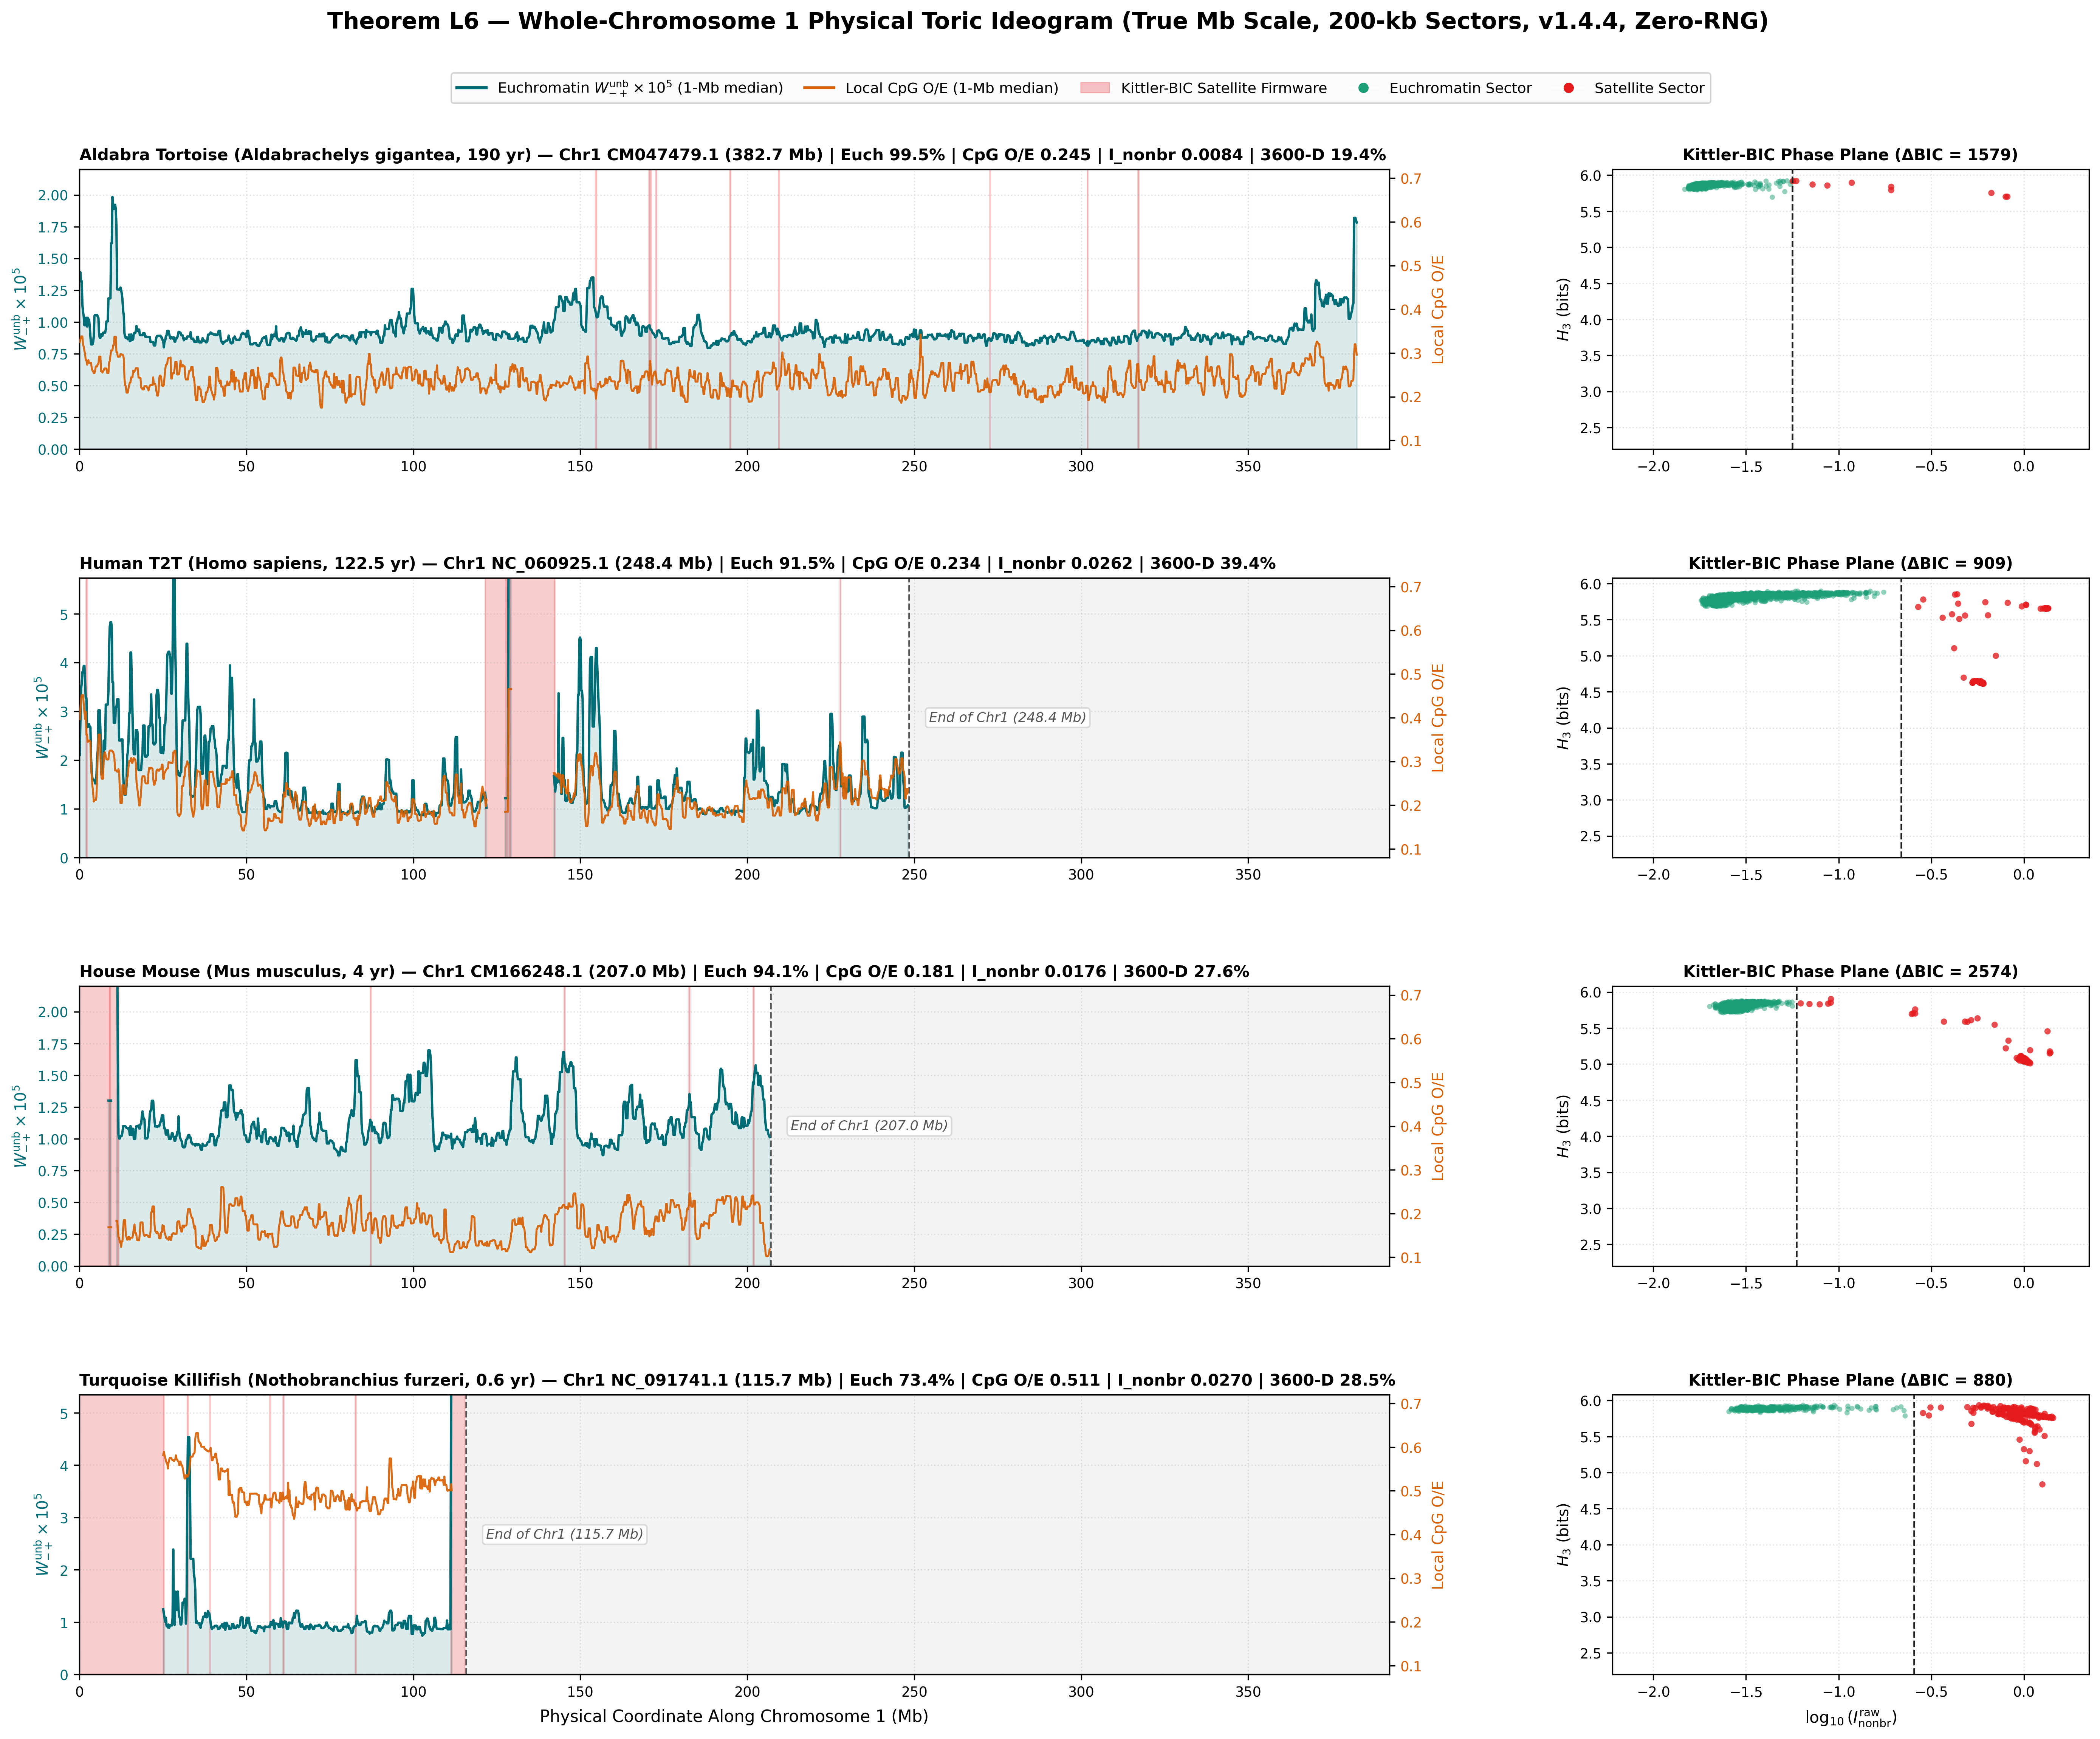
\includegraphics[width=\textwidth]{fig_L6_aldabra_vs_human_ideogram.png}
\caption{\textbf{Theorem~L6 --- Direct Four-Vertebrate Whole-Chromosome 1 Comparison (Aldabra Giant Tortoise vs.\ Human T2T, Mouse T2T, and Turquoise Killifish).}
Side-by-side 200-kb physical tracks of unbiased $W_{-+}^{\mathrm{unb}}$ (teal), local $\mathrm{CpG}$ O/E (orange), Kittler--BIC satellite bands (coral), and $(\log_{10} I_{\mathrm{nonbr}}^{\mathrm{raw}}, H_3)$ phase planes.}
\label{fig:L6}
\end{figure}

\begin{figure}[H]
\centering
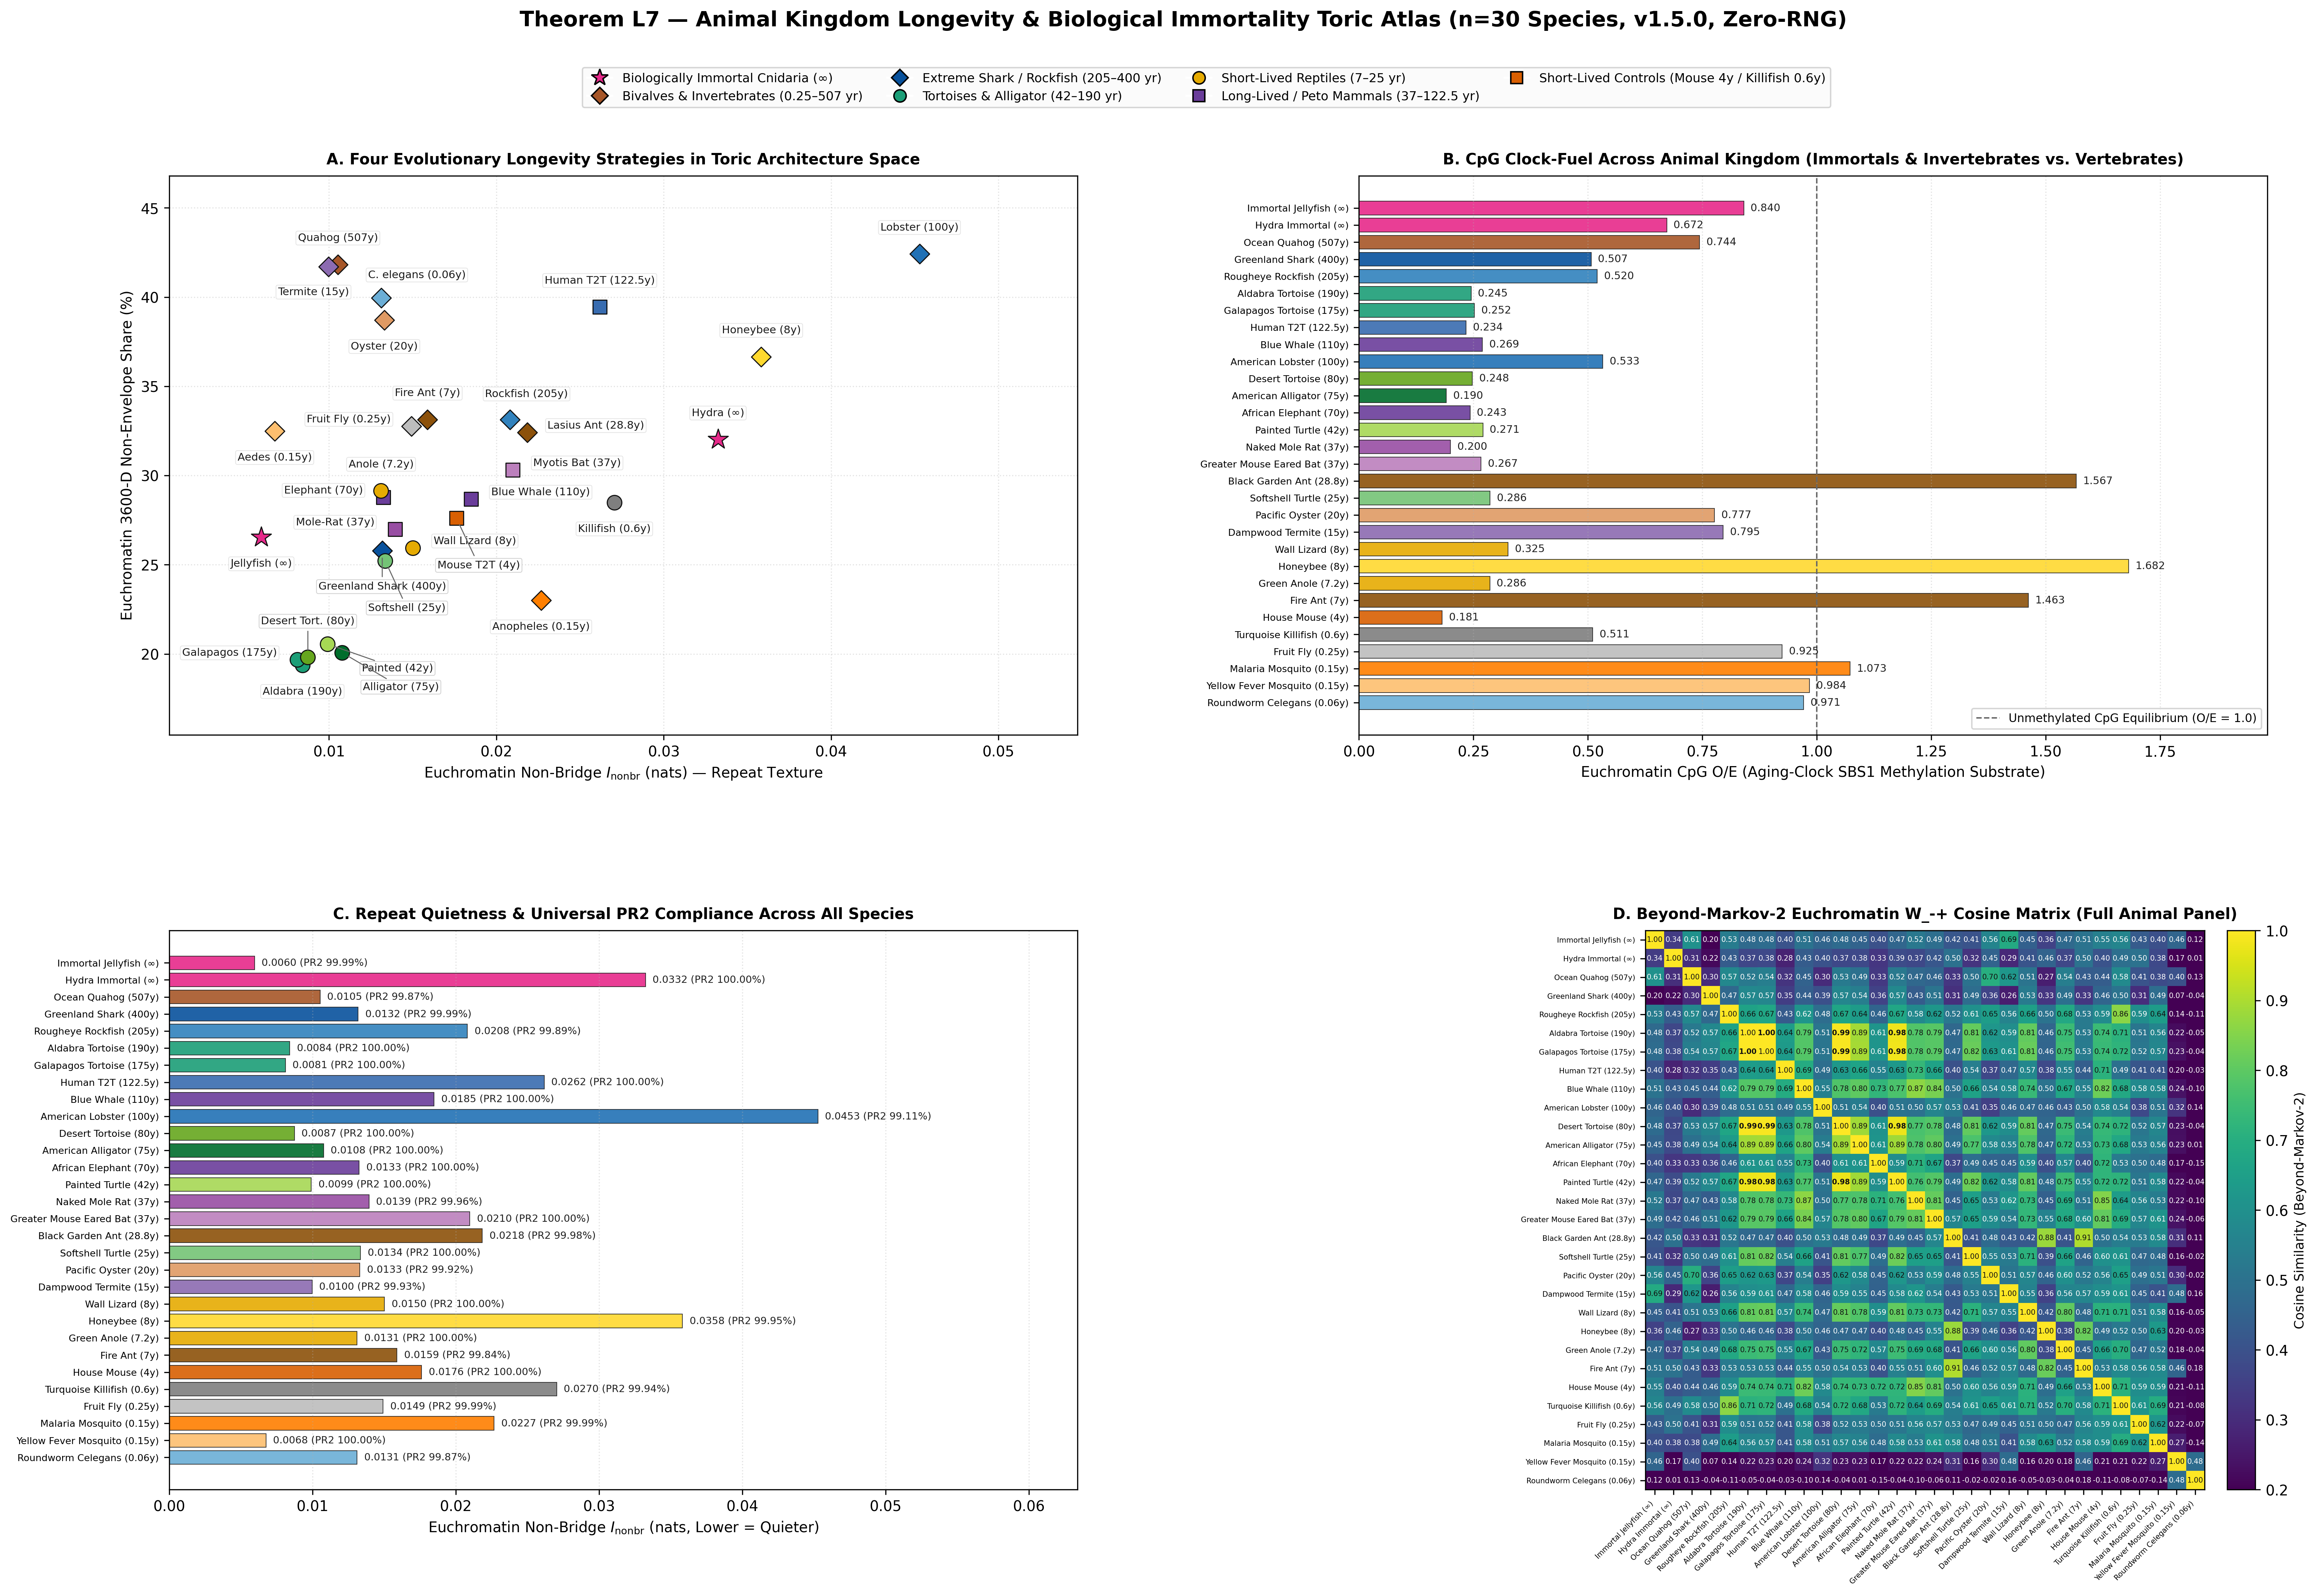
\includegraphics[width=\textwidth]{fig_L7_immortals_and_extremes_atlas.png}
\caption{\textbf{Theorem~L7 --- 30-Species Animal Kingdom Longevity and Biological Immortality Toric Atlas.}
(A) Evolutionary longevity strategies in $(I_{\mathrm{nonbr}}, \mathrm{3600\text{-}D})$ space: Archosaurian silence (bottom-left green cluster), Bivalvia/Termite/\textit{C.\ elegans} high-3600D cluster (top-left), active placental/human architecture, opposing immortal cnidarian poles (\textit{Turritopsis} vs.\ \textit{Hydra}), and the $100\text{-yr}$ American Lobster extreme (top-right).
(B) Euchromatin $\mathrm{CpG}$ O/E across all 30 species, highlighting Hymenopteran CpG hyper-enrichment ($1.463\text{--}1.682$) and unmethylated Diptera ($0.925\text{--}1.073$) exceeding both immortal cnidarians.
(C) Euchromatin repeat quietness $I_{\mathrm{nonbr}}$ and universal PR2 compliance ($99.11\text{--}100.00\%$).
(D) Full $30\times 30$ Beyond-Markov-2 euchromatin $W_{-+}$ cosine similarity matrix.}
\label{fig:L7}
\end{figure}

\begin{figure}[H]
\centering
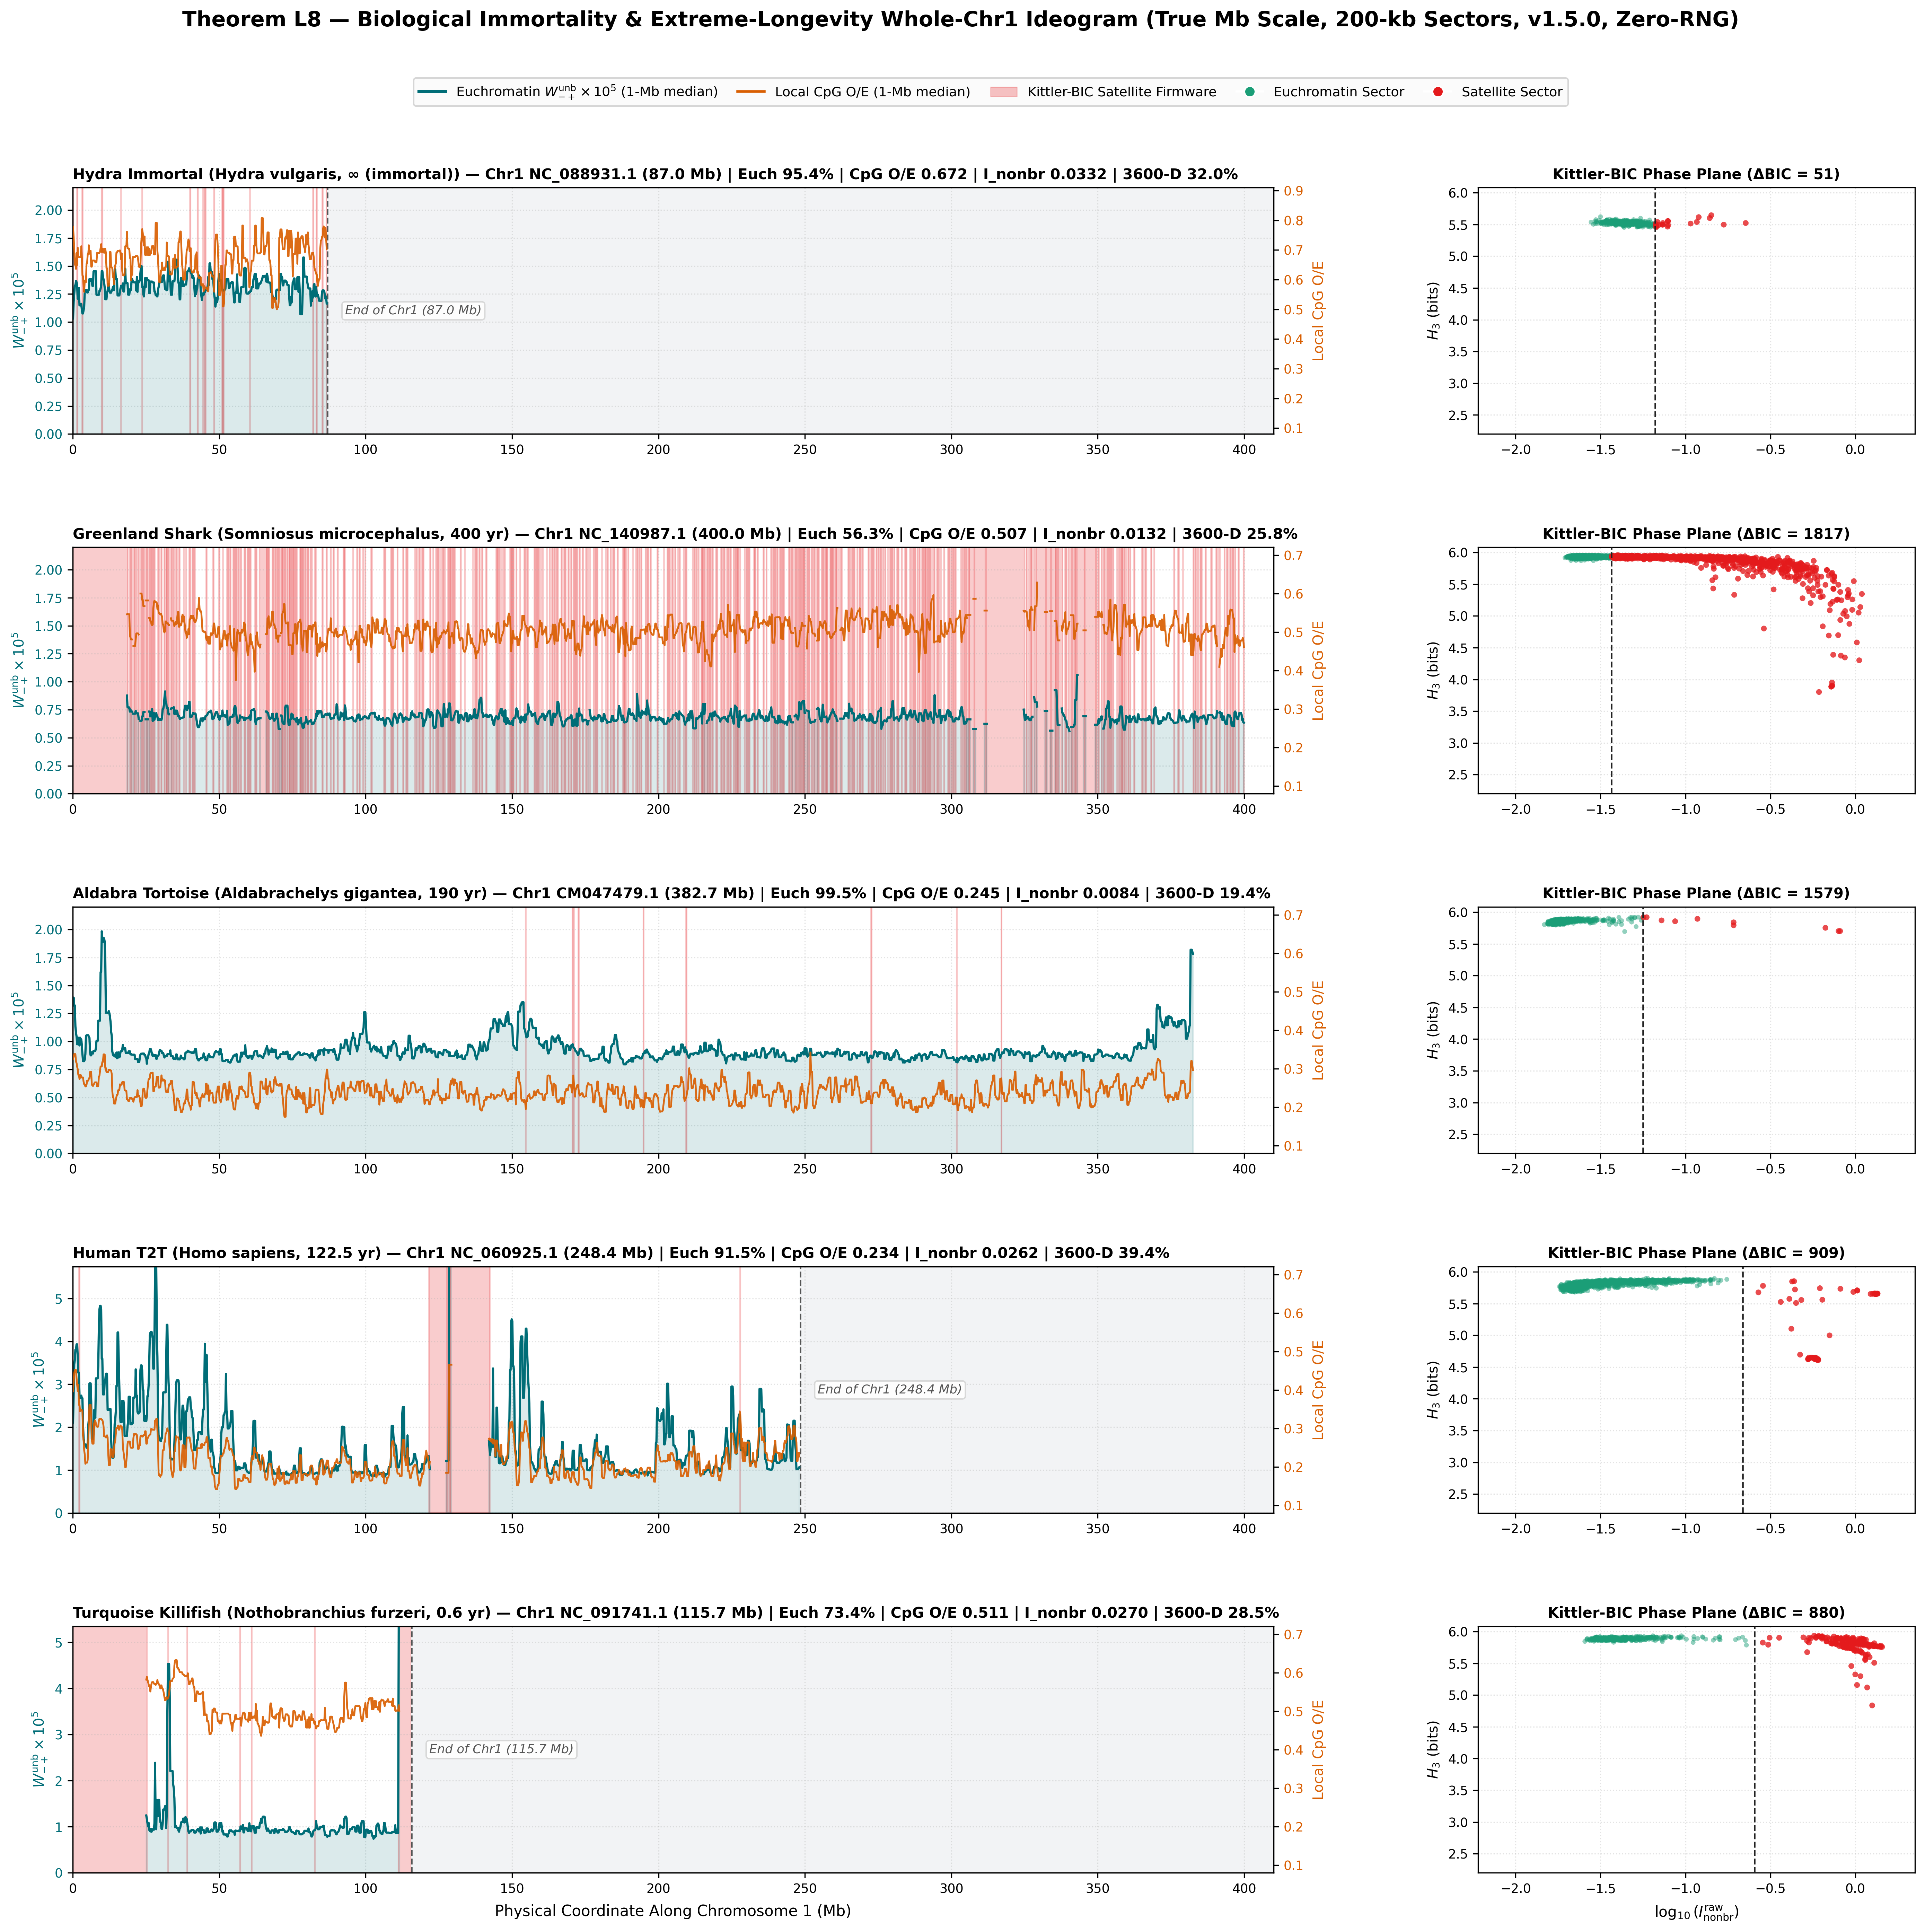
\includegraphics[width=\textwidth]{fig_L8_extremes_ideogram.png}
\caption{\textbf{Theorem~L8 --- True Physical Mb-Scale Whole-Chromosome Toric Ideogram Across Five Extreme Archetypes.}
From top to bottom: \textit{Hydra vulgaris} T2T ($\infty$, chr12, $87.0\text{ Mb}$, high $\mathrm{CpG}$ O/E $=0.672$, high $I_{\mathrm{nonbr}}=0.0332$), \textit{Somniosus microcephalus} ($400\text{ yr}$, $400.0\text{ Mb}$ prefix, $43.7\%$ interspersed Kittler--BIC satellite/repeat blocks, $\Delta\mathrm{BIC}=1817$), \textit{Aldabrachelys gigantea} ($190\text{ yr}$, $382.7\text{ Mb}$, $99.5\%$ serene euchromatin), \textit{Homo sapiens} T2T ($122.5\text{ yr}$, $248.4\text{ Mb}$, sharp centromeric satellite block and volatile Alu/LINE euchromatin), and \textit{Nothobranchius furzeri} ($0.6\text{ yr}$, $115.7\text{ Mb}$, $26.6\%$ satellite firmware).}
\label{fig:L8}
\end{figure}

% =====================================================================
\section{Track D: Multi-Lag Memory Spectrum, Null-Tower, Ecdysozoa Resonance, and the Toric Evolutionary Slowdown Clock (Theorems L8--L8g)}
% =====================================================================
Evaluating $I_{\mathrm{nonbr}}(d)$ across seven physical lags $d \in \{3, 6, 9, 10, 15, 30, 90\}\text{ bp}$ separates short-range local texture from persistent medium-range transposon/repeat fields across all 30 species (Table~\ref{tab:deep_l8}, Figure~\ref{fig:L9}A,C).
Three physical regimes emerge:
\begin{enumerate}
  \item \textbf{Ultra-rapid decay ($R_{\mathrm{mem}} \le 0.27$):} \textit{Anopheles gambiae} ($0.156$), \textit{Zootermopsis nevadensis} ($0.163$), \textit{Turritopsis dohrnii} ($0.194$, $I(90)=0.0005$), \textit{Pacific Oyster} ($0.220$), \textit{Rougheye Rockfish} ($0.225$), squamate lizards ($0.250\text{--}0.265$), and \textit{Fruit Fly} ($0.267$).
  \item \textbf{Serene low-amplitude archosaurian plateau ($I(3) \le 0.0108$, $R_{\mathrm{mem}} \approx 0.41\text{--}0.44$):} All four long-lived Cryptodira turtles and \textit{Alligator mississippiensis} cluster tightly in Figure~\ref{fig:L9}C with irreducible Beyond-Markov-2 energy shares of only $26.1\text{--}29.8\%$.
  \item \textbf{Persistent long-range repeat fields ($R_{\mathrm{mem}} > 0.51$):} \textit{Hydra vulgaris} ($0.573$), \textit{Homarus americanus} ($0.549$, highest absolute $I(3)=0.0452$ and $I(90)=0.0110$ in the entire 30-species atlas), \textit{Greenland Shark} ($0.525$, highest $I(90)/I(3) = 0.367$), and \textit{Human T2T} ($0.514$).
\end{enumerate}

\begin{table}[H]
\centering
{\renewcommand{\arraystretch}{0.88}
\caption{\textbf{Theorem~L8 --- Multi-Lag Euchromatin Memory Decay ($d=3\text{--}90\text{ bp}$), Exact Algebraic Null-Tower, and Intra-Chromosome Split-Half Reliability ($n=30$).} $R_{\mathrm{mem}} = I_{\mathrm{nonbr}}(30)/I_{\mathrm{nonbr}}(3)$ measures long-range repeat persistence; Beyond-M1/M2 give exact irreducible $W_{-+}$ energy shares above Markov-1 and Markov-2 compositional nulls; Split-Half $\cos_{\mathrm{M2}}(\mathrm{L},\mathrm{R}) \ge 0.9006$ across all 30 genomes ($27/30 \ge 0.95$).}
\label{tab:deep_l8}
\resizebox{\textwidth}{!}{%
\begin{tabular}{lrrrrrrrrrrr}
\toprule
\textbf{Species} & \textbf{Life} & \textbf{$I(3)$} & \textbf{$I(10)$} & \textbf{$I(30)$} & \textbf{$I(90)$} & \textbf{$R_{\mathrm{mem}}$} & \textbf{Bey-M1\%} & \textbf{Bey-M2\%} & \textbf{Pal\%} & \textbf{Split $\cos_{\mathrm{M2}}$} & \textbf{$\Delta$3600D} \\
\midrule
\textbf{Immortal Jellyfish} & $\infty$ & 0.0060 & 0.0023 & 0.0012 & 0.0005 & 0.194 & 33.2\% & 20.0\% & 3.97\% & 0.9900 & 0.17\,pp \\
\textbf{Hydra Immortal} & $\infty$ & 0.0332 & 0.0269 & 0.0190 & 0.0061 & 0.573 & 39.2\% & 55.7\% & 4.67\% & 0.9990 & 0.17\,pp \\
\textbf{Ocean Quahog} & 507 & 0.0105 & 0.0060 & 0.0032 & 0.0013 & 0.304 & 63.4\% & 45.8\% & 3.29\% & 0.9930 & 0.08\,pp \\
\textbf{Greenland Shark} & 400 & 0.0132 & 0.0081 & 0.0069 & 0.0048 & 0.525 & 48.9\% & 36.4\% & 2.59\% & 0.9849 & 1.45\,pp \\
\textbf{Rougheye Rockfish} & 205 & 0.0208 & 0.0109 & 0.0047 & 0.0018 & 0.225 & 67.7\% & 61.0\% & 3.15\% & 0.9852 & 0.88\,pp \\
\textbf{Aldabra Tortoise} & 190 & 0.0084 & 0.0053 & 0.0037 & 0.0024 & 0.443 & 38.2\% & 26.1\% & 3.05\% & 0.9942 & 0.80\,pp \\
\textbf{Galapagos Tortoise} & 175 & 0.0081 & 0.0049 & 0.0034 & 0.0021 & 0.413 & 38.3\% & 26.3\% & 3.15\% & 0.9946 & 0.92\,pp \\
\textbf{Human T2T} & 122.5 & 0.0262 & 0.0194 & 0.0134 & 0.0053 & 0.514 & 60.0\% & 63.1\% & 1.58\% & 0.9944 & 2.07\,pp \\
\textbf{Blue Whale} & 110 & 0.0185 & 0.0122 & 0.0078 & 0.0049 & 0.421 & 50.0\% & 58.6\% & 2.23\% & 0.9910 & 1.09\,pp \\
\textbf{American Lobster} & 100 & 0.0452 & 0.0299 & 0.0248 & 0.0110 & 0.549 & 78.3\% & 121.8\% & 1.96\% & 0.9289 & 2.17\,pp \\
\textbf{Desert Tortoise} & 80 & 0.0087 & 0.0055 & 0.0039 & 0.0026 & 0.443 & 38.0\% & 26.4\% & 3.06\% & 0.9941 & 1.12\,pp \\
\textbf{American Alligator} & 75 & 0.0108 & 0.0068 & 0.0046 & 0.0032 & 0.425 & 33.4\% & 27.9\% & 2.90\% & 0.9970 & 0.31\,pp \\
\textbf{African Elephant} & 70 & 0.0133 & 0.0093 & 0.0050 & 0.0026 & 0.374 & 41.6\% & 41.2\% & 1.66\% & 0.9809 & 3.48\,pp \\
\textbf{Painted Turtle} & 42 & 0.0099 & 0.0062 & 0.0044 & 0.0030 & 0.442 & 39.5\% & 29.8\% & 3.08\% & 0.9957 & 0.77\,pp \\
\textbf{Naked Mole Rat} & 37 & 0.0139 & 0.0089 & 0.0057 & 0.0032 & 0.406 & 46.1\% & 46.3\% & 1.92\% & 0.9818 & 1.31\,pp \\
\textbf{Greater Mouse Eared Bat} & 37 & 0.0210 & 0.0138 & 0.0085 & 0.0038 & 0.403 & 48.7\% & 66.7\% & 3.24\% & 0.9914 & 1.53\,pp \\
\textbf{Black Garden Ant} & 28.8 & 0.0218 & 0.0138 & 0.0079 & 0.0038 & 0.362 & 55.1\% & 58.4\% & 5.03\% & 0.9675 & 2.52\,pp \\
\textbf{Softshell Turtle} & 25 & 0.0134 & 0.0071 & 0.0047 & 0.0032 & 0.352 & 47.4\% & 37.9\% & 3.14\% & 0.9945 & 1.77\,pp \\
\textbf{Pacific Oyster} & 20 & 0.0133 & 0.0075 & 0.0029 & 0.0007 & 0.220 & 52.1\% & 40.2\% & 4.61\% & 0.9867 & 1.11\,pp \\
\textbf{Dampwood Termite} & 15 & 0.0100 & 0.0036 & 0.0016 & 0.0005 & 0.163 & 83.1\% & 50.2\% & 1.88\% & 0.9937 & 0.42\,pp \\
\textbf{Wall Lizard} & 8 & 0.0150 & 0.0069 & 0.0038 & 0.0018 & 0.250 & 44.6\% & 36.7\% & 3.51\% & 0.9941 & 0.30\,pp \\
\textbf{Honeybee} & 8 & 0.0359 & 0.0162 & 0.0102 & 0.0066 & 0.283 & 53.8\% & 67.3\% & 7.28\% & 0.9818 & 6.20\,pp \\
\textbf{Green Anole} & 7.2 & 0.0131 & 0.0072 & 0.0035 & 0.0017 & 0.265 & 50.4\% & 36.2\% & 2.83\% & 0.9957 & 1.12\,pp \\
\textbf{Fire Ant} & 7 & 0.0160 & 0.0117 & 0.0074 & 0.0045 & 0.461 & 48.4\% & 51.7\% & 6.30\% & 0.9259 & 0.02\,pp \\
\textbf{House Mouse} & 4 & 0.0176 & 0.0127 & 0.0064 & 0.0023 & 0.364 & 42.2\% & 53.1\% & 2.19\% & 0.9973 & 0.64\,pp \\
\textbf{Turquoise Killifish} & 0.6 & 0.0270 & 0.0178 & 0.0105 & 0.0037 & 0.388 & 62.3\% & 56.9\% & 4.08\% & 0.9854 & 1.62\,pp \\
\textbf{Fruit Fly} & 0.25 & 0.0149 & 0.0082 & 0.0040 & 0.0018 & 0.267 & 65.6\% & 70.0\% & 3.74\% & 0.9909 & 1.42\,pp \\
\textbf{Malaria Mosquito} & 0.15 & 0.0227 & 0.0109 & 0.0035 & 0.0020 & 0.156 & 59.9\% & 76.5\% & 4.23\% & 0.9920 & 0.18\,pp \\
\textbf{Yellow Fever Mosquito} & 0.15 & 0.0068 & 0.0057 & 0.0023 & 0.0012 & 0.335 & 40.4\% & 18.3\% & 6.25\% & 0.9951 & 0.12\,pp \\
\textbf{Roundworm (\textit{C.\ elegans})} & 0.06 & 0.0132 & 0.0077 & 0.0045 & 0.0018 & 0.343 & 39.7\% & 11.4\% & 4.83\% & 0.9006 & 4.11\,pp \\
\bottomrule
\end{tabular}}}
\end{table}

\subsection{The Toric Evolutionary Slowdown Clock}
Normalizing Beyond-Markov-2 toric distance $d_{\mathrm{toric}} = 1 - \cos_{\mathrm{Beyond\text{-}M2}}$ by consensus divergence time $T_{\mathrm{div}}$ (in units of $100\text{ Myr}$) yields an exact structural drift rate across 17 independent clade pairs spanning Deuterostomia, Lophotrochozoa, and Ecdysozoa (Table~\ref{tab:clock_l8}, Figure~\ref{fig:L9}B).
Long-lived Cryptodira tortoises drift at only \textbf{$0.0075\text{--}0.0238$ per $100\text{ Myr}$} ($\cos = 0.9972$ over $38\text{ Myr}$ between Aldabra and Galapagos; $\cos = 0.9805$ over $82\text{ Myr}$ between Aldabra and Painted Turtle), and across the $255\text{-Myr}$ Archelosauria split between \textit{Aldabrachelys gigantea} and \textit{Alligator mississippiensis}, Beyond-Markov-2 alignment remains $\cos = 0.8901$ ($0.0431$ per $100\text{ Myr}$).
Eusocial Hymenoptera also exhibit slow structural drift (\textit{Apis} $\times$ \textit{Lasius}, $160\text{ Myr}$: $0.0765$ per $100\text{ Myr}$; \textit{Lasius} $\times$ \textit{Solenopsis}, $100\text{ Myr}$: $0.0969$), comparable to the $460\text{-Myr}$ Bivalvia split ($0.0650$).
By contrast, placental mammals separated by $<100\text{ Myr}$ diverge $10\text{--}60\times$ faster than Cryptodira ($0.3261\text{--}0.4499$ per $100\text{ Myr}$; $13\text{--}79\times$ under saturation-corrected $-\ln(\cos_{\mathrm{M2}})/100\text{ Myr}$).
Remarkably, the single fastest structural drift rate in the entire 17-pair atlas occurs inside a single mosquito family---Culicidae (\textit{Anopheles gambiae} $\times$ \textit{Aedes aegypti}, $150\text{ Myr}$, $\cos = 0.2679$, drift \textbf{$0.4881$ per $100\text{ Myr}$})---exceeding even \textit{Human} $\times$ \textit{Elephant} ($0.4499$), directly quantifying how massive transposable-element genome inflation in \textit{Aedes} ($474\text{ Mb}$ chr2 vs.\ $118\text{ Mb}$ in \textit{Anopheles}) rapidly rewrites higher-order Beyond-Markov-2 syntax.

\begin{table}[H]
\centering
\caption{\textbf{The Toric Evolutionary Slowdown Clock (Theorem~L8, 17 Clade Pairs).} Beyond-Markov-2 structural drift rate $(1-\cos_{\mathrm{M2}})/100\text{ Myr}$ across 17 TimeTree-calibrated clade pairs. Long-lived Cryptodira turtles and Archelosauria anchor the ultra-slow stasis regime ($0.0075\text{--}0.0431$), whereas transposon-expanded Culicidae (\textit{Anopheles} $\times$ \textit{Aedes}, $0.4881$) and placental mammals ($0.3261\text{--}0.4499$) occupy the rapid-remodeling regime.}
\label{tab:clock_l8}
\resizebox{\textwidth}{!}{%
\begin{tabular}{llrrrr}
\toprule
\textbf{Calibrated Species Pair} & \textbf{Clade} & \textbf{Div.\ (Myr)} & \textbf{$\cos_{\mathrm{Beyond\text{-}M2}}$} & \textbf{Toric Dist.\ $(1-\cos)$} & \textbf{Drift / 100 Myr} \\
\midrule
Aldabra Tortoise $\times$ Galapagos Tortoise & Testudines (Giant Tortoises) & 38 & 0.9972 & 0.0028 & \textbf{0.0075} \\
Aldabra Tortoise $\times$ Desert Tortoise & Testudines (Tortoises) & 55 & 0.9926 & 0.0074 & \textbf{0.0135} \\
Aldabra Tortoise $\times$ Painted Turtle & Testudines (Cryptodira) & 82 & 0.9805 & 0.0195 & \textbf{0.0238} \\
Aldabra Tortoise $\times$ American Alligator & Archelosauria & 255 & 0.8901 & 0.1099 & \textbf{0.0431} \\
Ocean Quahog $\times$ Pacific Oyster & Bivalvia (507y vs 20y) & 460 & 0.7008 & 0.2992 & \textbf{0.0650} \\
Honeybee $\times$ Black Garden Ant & Aculeata (Bee vs Ant) & 160 & 0.8776 & 0.1224 & \textbf{0.0765} \\
Black Garden Ant $\times$ Fire Ant & Formicidae (Lasius vs Fire Ant) & 100 & 0.9031 & 0.0969 & 0.0969 \\
Aldabra Tortoise $\times$ Softshell Turtle & Testudines (Deep) & 160 & 0.8112 & 0.1888 & 0.1180 \\
Wall Lizard $\times$ Green Anole & Squamata (Lizards) & 165 & 0.8034 & 0.1966 & 0.1192 \\
Rougheye Rockfish $\times$ Turquoise Killifish & Teleostei (205y vs 0.6y) & 115 & 0.8591 & 0.1409 & 0.1226 \\
Fruit Fly $\times$ Malaria Mosquito & Diptera (Fly vs Anopheles) & 260 & 0.6225 & 0.3775 & 0.1452 \\
Naked Mole Rat $\times$ House Mouse & Rodentia (Mole-Rat vs Mouse) & 70 & 0.8510 & 0.1490 & 0.2129 \\
Human T2T $\times$ Blue Whale & Boreoeutheria (Human-Whale) & 94 & 0.6935 & 0.3065 & 0.3261 \\
Human T2T $\times$ House Mouse & Euarchontoglires & 87 & 0.7113 & 0.2887 & 0.3318 \\
Human T2T $\times$ Greater Mouse Eared Bat & Boreoeutheria (Human-Bat) & 94 & 0.6626 & 0.3374 & 0.3589 \\
Human T2T $\times$ African Elephant & Placentalia (Human-Elephant) & 99 & 0.5546 & 0.4454 & 0.4499 \\
Malaria Mosquito $\times$ Yellow Fever Mosquito & Culicidae (Anopheles vs Aedes) & 150 & 0.2679 & 0.7321 & \textbf{0.4881} \\
\bottomrule
\end{tabular}}
\end{table}

\subsection{Isotropy Quanta (\texorpdfstring{$447/512$}{447/512} and \texorpdfstring{$1/32$}{1/32}), Sauropsid Fidelity, Mammalian Overshoot, and Ecdysozoa Physics (Theorems L8b--L8g)}
\begin{theorem}[Asymptotic $447/512$ Isotropy Relaxation Across 30 Species]
\label{thm:L8b}
While adjacent triplets ($d=3\text{ bp}$) confine $57.6\text{--}80.6\%$ of $W_{-+}$ energy inside the $130\text{-D}$ boundary screen ($\mathrm{3600\text{-}D} = 19.4\text{--}42.4\%$, tightest in Archosauria at $19.4\text{--}20.6\%$), breaking the direct dinucleotide junction at $d=30\text{ bp}$ drives $27$ of $30$ species asymptotically toward the exact geometric isotropy limit $447/512 = 87.30\%$ of Theorem~\ref{thm:env496} ($\mathrm{3600\text{-}D}(30) \in [71.2\%, 85.9\%]$, peaking at $85.94\%$ in \textit{Homarus americanus}, just $1.36\text{ pp}$ below the exact theoretical ceiling, while debiased $W_{-+}^{\mathrm{unb}}(30)$ remains far above the $1/(4N)$ finite-sample floor). The only three genomes remaining below $65\%$ at $d=30\text{ bp}$ are the two compact Diptera (\textit{Anopheles gambiae} $48.3\%$, \textit{Drosophila melanogaster} $57.0\%$) and \textit{Caenorhabditis elegans} ($60.6\%$; Figure~\ref{fig:L10}A).
\end{theorem}

\begin{theorem}[Exact $1/32$ Palindromic Isotropy Quantum, Mammalian Depletion, and Hymenopteran Hyper-Palindromes]
\label{thm:L8c}
By Theorem~\ref{thm:sbs1_pal}, isotropic distribution of $W_{-+}$ energy predicts an exact palindromic share $\mathrm{Iso}_{\mathrm{pal}}(W_{-+}) = 32/1024 = 1/32 = 3.125\%$. Across the $30$-species panel, all five Testudines remain tightly locked onto this zero-parameter quantum ($3.05\text{--}3.15\%$), whereas five of six placental mammals actively deplete palindromic $W_{-+}$ energy to $0.51\text{--}0.71\times\frac{1}{32}$ (Human $1.58\%$, Elephant $1.66\%$, Mole-Rat $1.92\%$, Mouse $2.19\%$, Blue Whale $2.23\%$; mammalian median $2.05\%$ vs.\ $24$ non-mammals median $3.40\%$; exact DP Mann--Whitney $U_1 = 16/144$, $r_{\mathrm{rb}} = -0.778$, $p = 2.14 \times 10^{-3}$), with \textit{Myotis myotis} ($3.24\%$) as the sole mammalian exception, joined below $2\%$ among invertebrates only by \textit{Zootermopsis} ($1.88\%$) and \textit{Homarus} ($1.96\%$). At the opposite pole, hyper-CpG Hymenoptera (\textit{Apis mellifera} $7.28\% = 2.33\times\frac{1}{32}$, \textit{Solenopsis invicta} $6.30\%$, \textit{Lasius niger} $5.03\%$) and \textit{Aedes aegypti} ($6.25\%$) strongly enrich chirally immune palindromic orbits (Figure~\ref{fig:L10}C).
\end{theorem}

\begin{theorem}[Sauropsid Markov-2 Cosine Fidelity Law and Short-Range Silence]
\label{thm:L8d}
Across all $n=8$ sauropsids, the cosine alignment $\cos_{\mathrm{M2}} = \cos(W_{-+}, W_{-+}(P_{\mathrm{M2}}))$ increases strictly monotonically with maximum lifespan from \textit{Anolis carolinensis} ($0.8128$, $7.2\text{ yr}$) and \textit{Podarcis muralis} ($0.8146$, $8\text{ yr}$) through \textit{Pelodiscus sinensis} ($0.8168$, $25\text{ yr}$), \textit{Chrysemys picta} ($0.8641$, $42\text{ yr}$), \textit{Alligator mississippiensis} ($0.8723$, $75\text{ yr}$), \textit{Gopherus evgoodei} ($0.8769$, $80\text{ yr}$), and \textit{Chelonoidis abingdonii} ($0.8787$, $175\text{ yr}$) to \textit{Aldabrachelys gigantea} ($0.8798$, $190\text{ yr}$), yielding $\rho_S(\cos_{\mathrm{M2}}, \text{Life}) = +1.000$ (exact permutation $p = 4.96 \times 10^{-5}$; equivalently $\sin^2\theta_{\mathrm{M2}} = 33.93\% \to 22.60\%$), while inside Archelosauria ($n=6$) raw Beyond-M2 energy decreases strictly monotonically ($37.95\% \to 26.14\%$, $\rho_S = -1.000$, $p = 2.78 \times 10^{-3}$). Crucially, $90\text{-bp}$ memory $I_{\mathrm{nonbr}}(90)$ is higher in long-lived sauropsids ($0.0021\text{--}0.0032$) than in lizards ($0.0017\text{--}0.0018$) and $R_{\mathrm{mem}}(30/3)$ increases with lifespan ($\rho_S = +0.762$, $p = 0.0280$), demonstrating that Archosaurian silence is specifically a short-range ($d \le 10\text{ bp}$) local repeat suppression rather than erasure of $90\text{-bp}$ correlations.
\end{theorem}

\begin{theorem}[Mammalian Markov-2 Radial Overshoot Inversion]
\label{thm:L8e}
By Proposition~\ref{prop:radial_angular}, the residual shift $\Delta_{\mathrm{M2\text{-}M1}} = E_{\mathrm{M2}} - E_{\mathrm{M1}}$ turns positive whenever radial projection overshoot outweighs a weak angular gain $\Delta\cos_{\mathrm{M2\text{-}M1}}$. Across all $17$ mortal vertebrates, placental mammals ($n_1=6$: $\Delta_{\mathrm{M2\text{-}M1}} \in [-0.35, +18.00]\text{ pp}$, median $+5.81\text{ pp}$) separate with zero overlap (gap $5.03\text{ pp}$) from all $11$ non-mammalian vertebrates ($\Delta_{\mathrm{M2\text{-}M1}} \in [-14.21, -5.39]\text{ pp}$, median $-9.70\text{ pp}$; exact DP $U_1 = 66/66$, $r_{\mathrm{rb}} = +1.000$, $p = 2/\binom{17}{6} = 1.62 \times 10^{-4}$), and equivalently in angular gain $\Delta\cos_{\mathrm{M2\text{-}M1}}$ ($U_1 = 0/66$, $r_{\mathrm{rb}} = -1.000$, $p = 1.62 \times 10^{-4}$). Across the full $30$-species panel ($n_1=6$ vs.\ $n_2=24$ non-mammals), both separations persist ($\Delta E$: $U_1 = 114/144$, $r_{\mathrm{rb}} = +0.583$, DP $p = 2.86 \times 10^{-2}$; $\Delta\cos$: $U_1 = 16/144$, $r_{\mathrm{rb}} = -0.778$, DP $p = 2.14 \times 10^{-3}$), while compact or repeat-structured arthropods (\textit{Homarus} $+43.5\text{ pp}$ to $E_{\mathrm{M2}}=121.8\%$, \textit{Anopheles} $+16.6\text{ pp}$, \textit{Apis} $+13.6\text{ pp}$, \textit{Drosophila} $+4.5\text{ pp}$, ants $+3.3\text{ pp}$) demonstrate that Markov-2 radial overshoot also arises independently in Ecdysozoa.
\end{theorem}

\begin{theorem}[Ecdysozoa $10\text{-bp}$ Compact-Diptera Resonance, Hymenopteran CpG Anti-Mirage, and \textit{C.\ elegans} Orthogonality]
\label{thm:L8g}
Auditing nine Ecdysozoa spanning Diptera, Hymenoptera, Blattodea, Crustacea, and Nematoda resolves four lineage-specific physical mechanisms:
\begin{enumerate}
  \item \textbf{Compact-Diptera nucleosome screen lock vs.\ transposon release:} \textit{Drosophila melanogaster} remains the unique species among all $30$ whose $3600\text{-D}$ share drops below $d=3\text{ bp}$ at $d=10\text{ bp}$ ($32.7\% \to 29.9\%$, $\Delta = -2.87\text{ pp}$), while its compact sister \textit{Anopheles gambiae} exhibits a matching local dip ($d=9$: $37.3\% \to d=10$: $35.5\%$) and both compact Diptera remain trapped far below the $447/512$ ceiling through $d=90\text{ bp}$ ($47.6\%$ and $39.3\%$) with strong $10.2\text{--}10.4\text{ bp}$ WW--SS antiphase phasing ($171.4^\circ\text{--}176.9^\circ$, $p_{\mathrm{adj}} \le 1.39\times 10^{-12}$) and elevated Beyond-M2 energy ($70.0\text{--}76.5\%$). Expanding the Dipteran genome with transposable elements in \textit{Aedes aegypti} ($474\text{ Mb}$ chr2) completely abolishes the screen lock ($\mathrm{3600\text{-}D}(30)=81.1\%$, $\mathrm{3600\text{-}D}(90)=81.8\%$, Beyond-M2 $= 18.3\%$).
  \item \textbf{Hymenopteran CpG hyper-enrichment and compositional anti-mirage:} All three Hymenoptera strongly enrich euchromatin $\mathrm{CpG}$ above equilibrium (\textit{Apis mellifera} $1.682$, \textit{Lasius niger} $1.567$, \textit{Solenopsis invicta} $1.463$), in sharp contrast to independently eusocial \textit{Zootermopsis nevadensis} ($0.795$, Blattodea) and \textit{Homarus americanus} ($0.533$). This produces the exact mirror image of the cnidarian compositional mirage: in raw $W_{-+}$, Hymenoptera appear orthogonal to vertebrates ($\cos_{W_{-+}}(\text{Honeybee}, \text{Aldabra}) = -0.015$, $\cos_{W_{-+}}(\text{Lasius}, \text{Aldabra}) = +0.015$), but subtracting the stationary Markov-2 null \emph{restores} hidden shared higher-order alignment by $+0.46\text{ to }+0.48$ ($\cos_{\mathrm{Beyond\text{-}M2}} = +0.464\text{ and }+0.471$).
  \item \textbf{Lobster extreme repeat tolerance and GC-orbit convergence:} The negligibly senescent $100\text{-yr}$ American lobster (\textit{Homarus americanus}) sets the 30-species maxima in $I_{\mathrm{nonbr}}(3)=0.0452$, $\mathrm{3600\text{-}D}(3)=42.4\%$, $\mathrm{3600\text{-}D}(30)=85.94\%$, and Beyond-M2 $=121.8\%$, and is the only non-human species whose top-5 $W_{-+}$ flux contains the GC-rich purine/pyrimidine orbit \texttt{GGG-AGG} ($2.6\%$, rank~\#2; Appendix~\ref{app:motifs}).
  \item \textbf{\textit{C.\ elegans} orthogonal island:} \textit{Caenorhabditis elegans} ($0.06\text{ yr}$, chrV) exhibits a $3.3\text{--}8.6\times$ larger directed time-arrow amplitude than every other species ($W_{-+}^{\mathrm{unb}} = 4.47\times 10^{-5}$ vs.\ $0.52\text{--}1.34\times 10^{-5}$ across the other $29$), minimal Beyond-M2 share ($11.4\%$), near-zero or negative Beyond-M2 cosine against all $17$ vertebrates ($\cos_{\mathrm{Beyond\text{-}M2}} \in [-0.147, +0.009]$; $-0.047$ vs.\ Aldabra, $-0.026$ vs.\ Human), and positive alignment exclusively with AT-tract-rich \textit{Aedes} ($+0.481$).
\end{enumerate}
\end{theorem}

\begin{figure}[H]
\centering
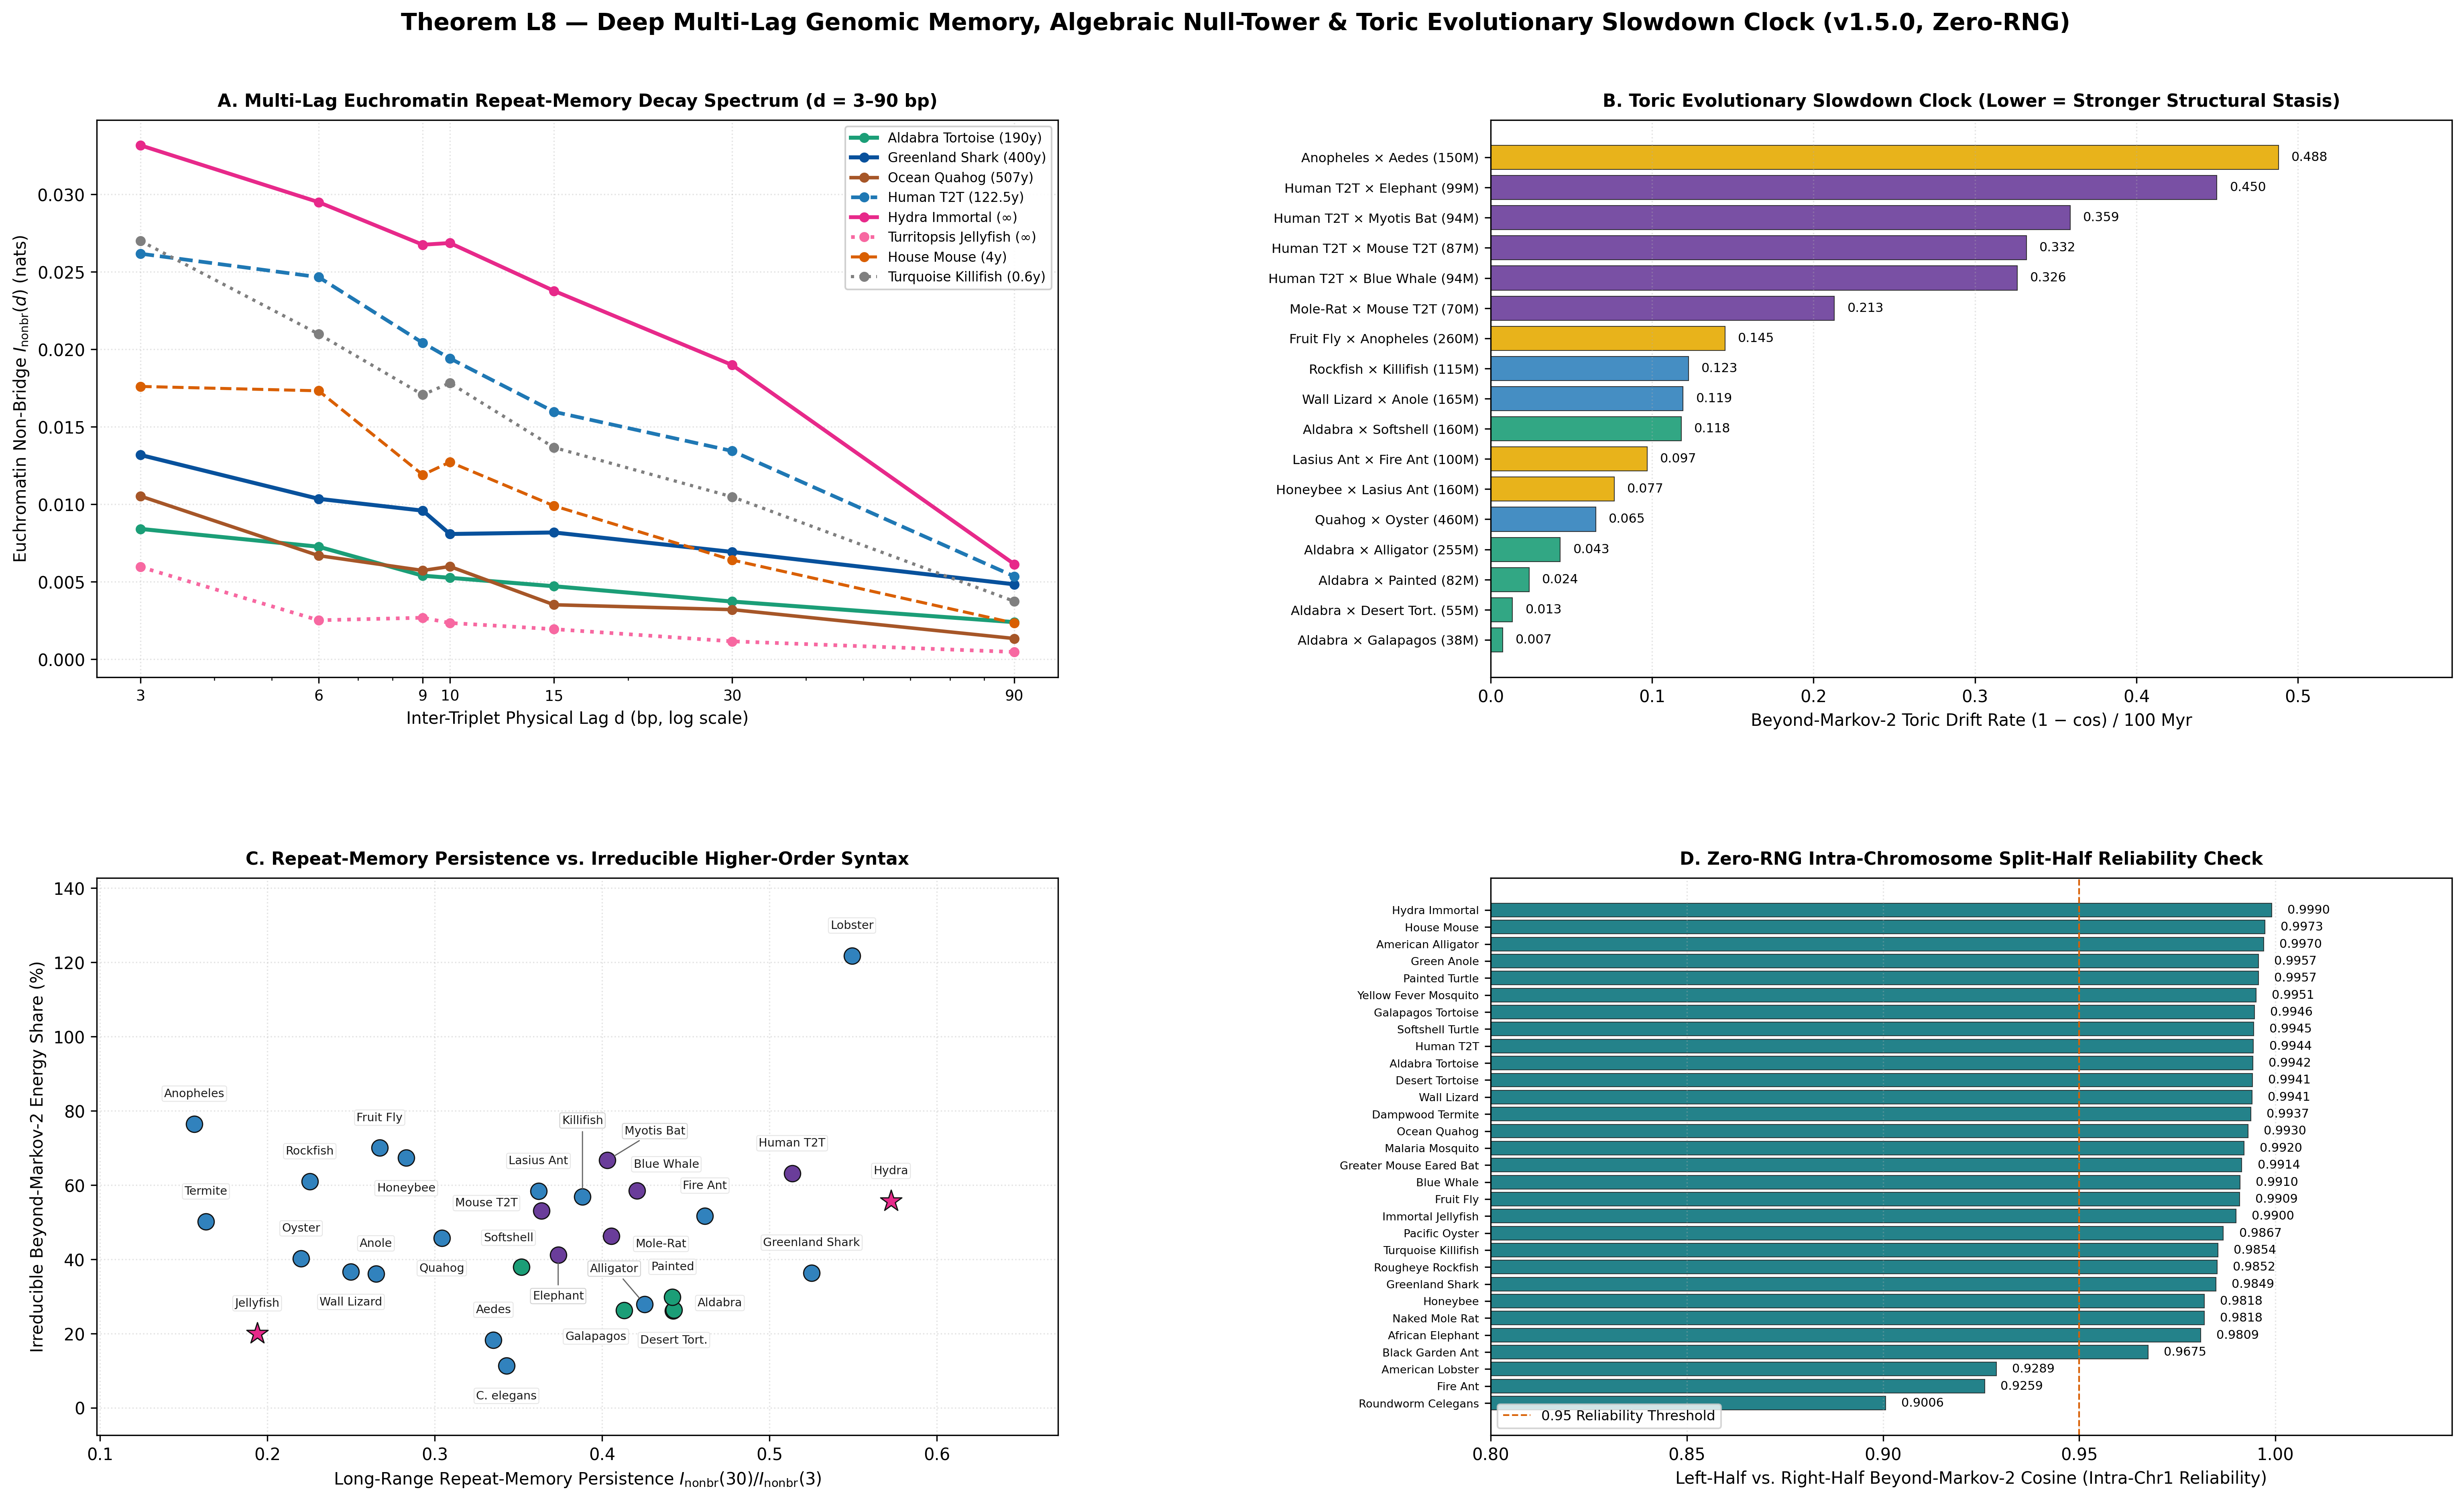
\includegraphics[width=\textwidth]{fig_L9_deep_memory_and_evolutionary_clock.png}
\caption{\textbf{Theorem~L8 --- Multi-Lag Memory Decay, Toric Evolutionary Slowdown Clock, Null-Tower Phase Map, and Split-Half Reliability ($n=30$).}
(A) Multi-lag euchromatin $I_{\mathrm{nonbr}}(d)$ decay curves ($d=3\text{--}90\text{ bp}$) contrasting serene \textit{Turritopsis} and giant tortoises against persistent \textit{Hydra}, \textit{Human T2T}, and \textit{Greenland Shark}.
(B) Beyond-Markov-2 Toric Evolutionary Slowdown Clock across 17 calibrated clade pairs showing Archosaurian/Bivalve/Hymenopteran stasis versus rapid remodeling in placental mammals and transposon-expanded Culicidae (\textit{Anopheles} $\times$ \textit{Aedes}, $0.488$).
(C) Long-range persistence $R_{\mathrm{mem}}(30/3)$ versus irreducible Beyond-Markov-2 energy share showing the tight Archosaurian cluster, \textit{Homarus} overshoot peak ($121.8\%$), and \textit{C.\ elegans} floor ($11.4\%$).
(D) Zero-RNG intra-chromosome split-half reliability across all 30 genomes ($27/30 \ge 0.95$).}
\label{fig:L9}
\end{figure}

\begin{figure}[H]
\centering
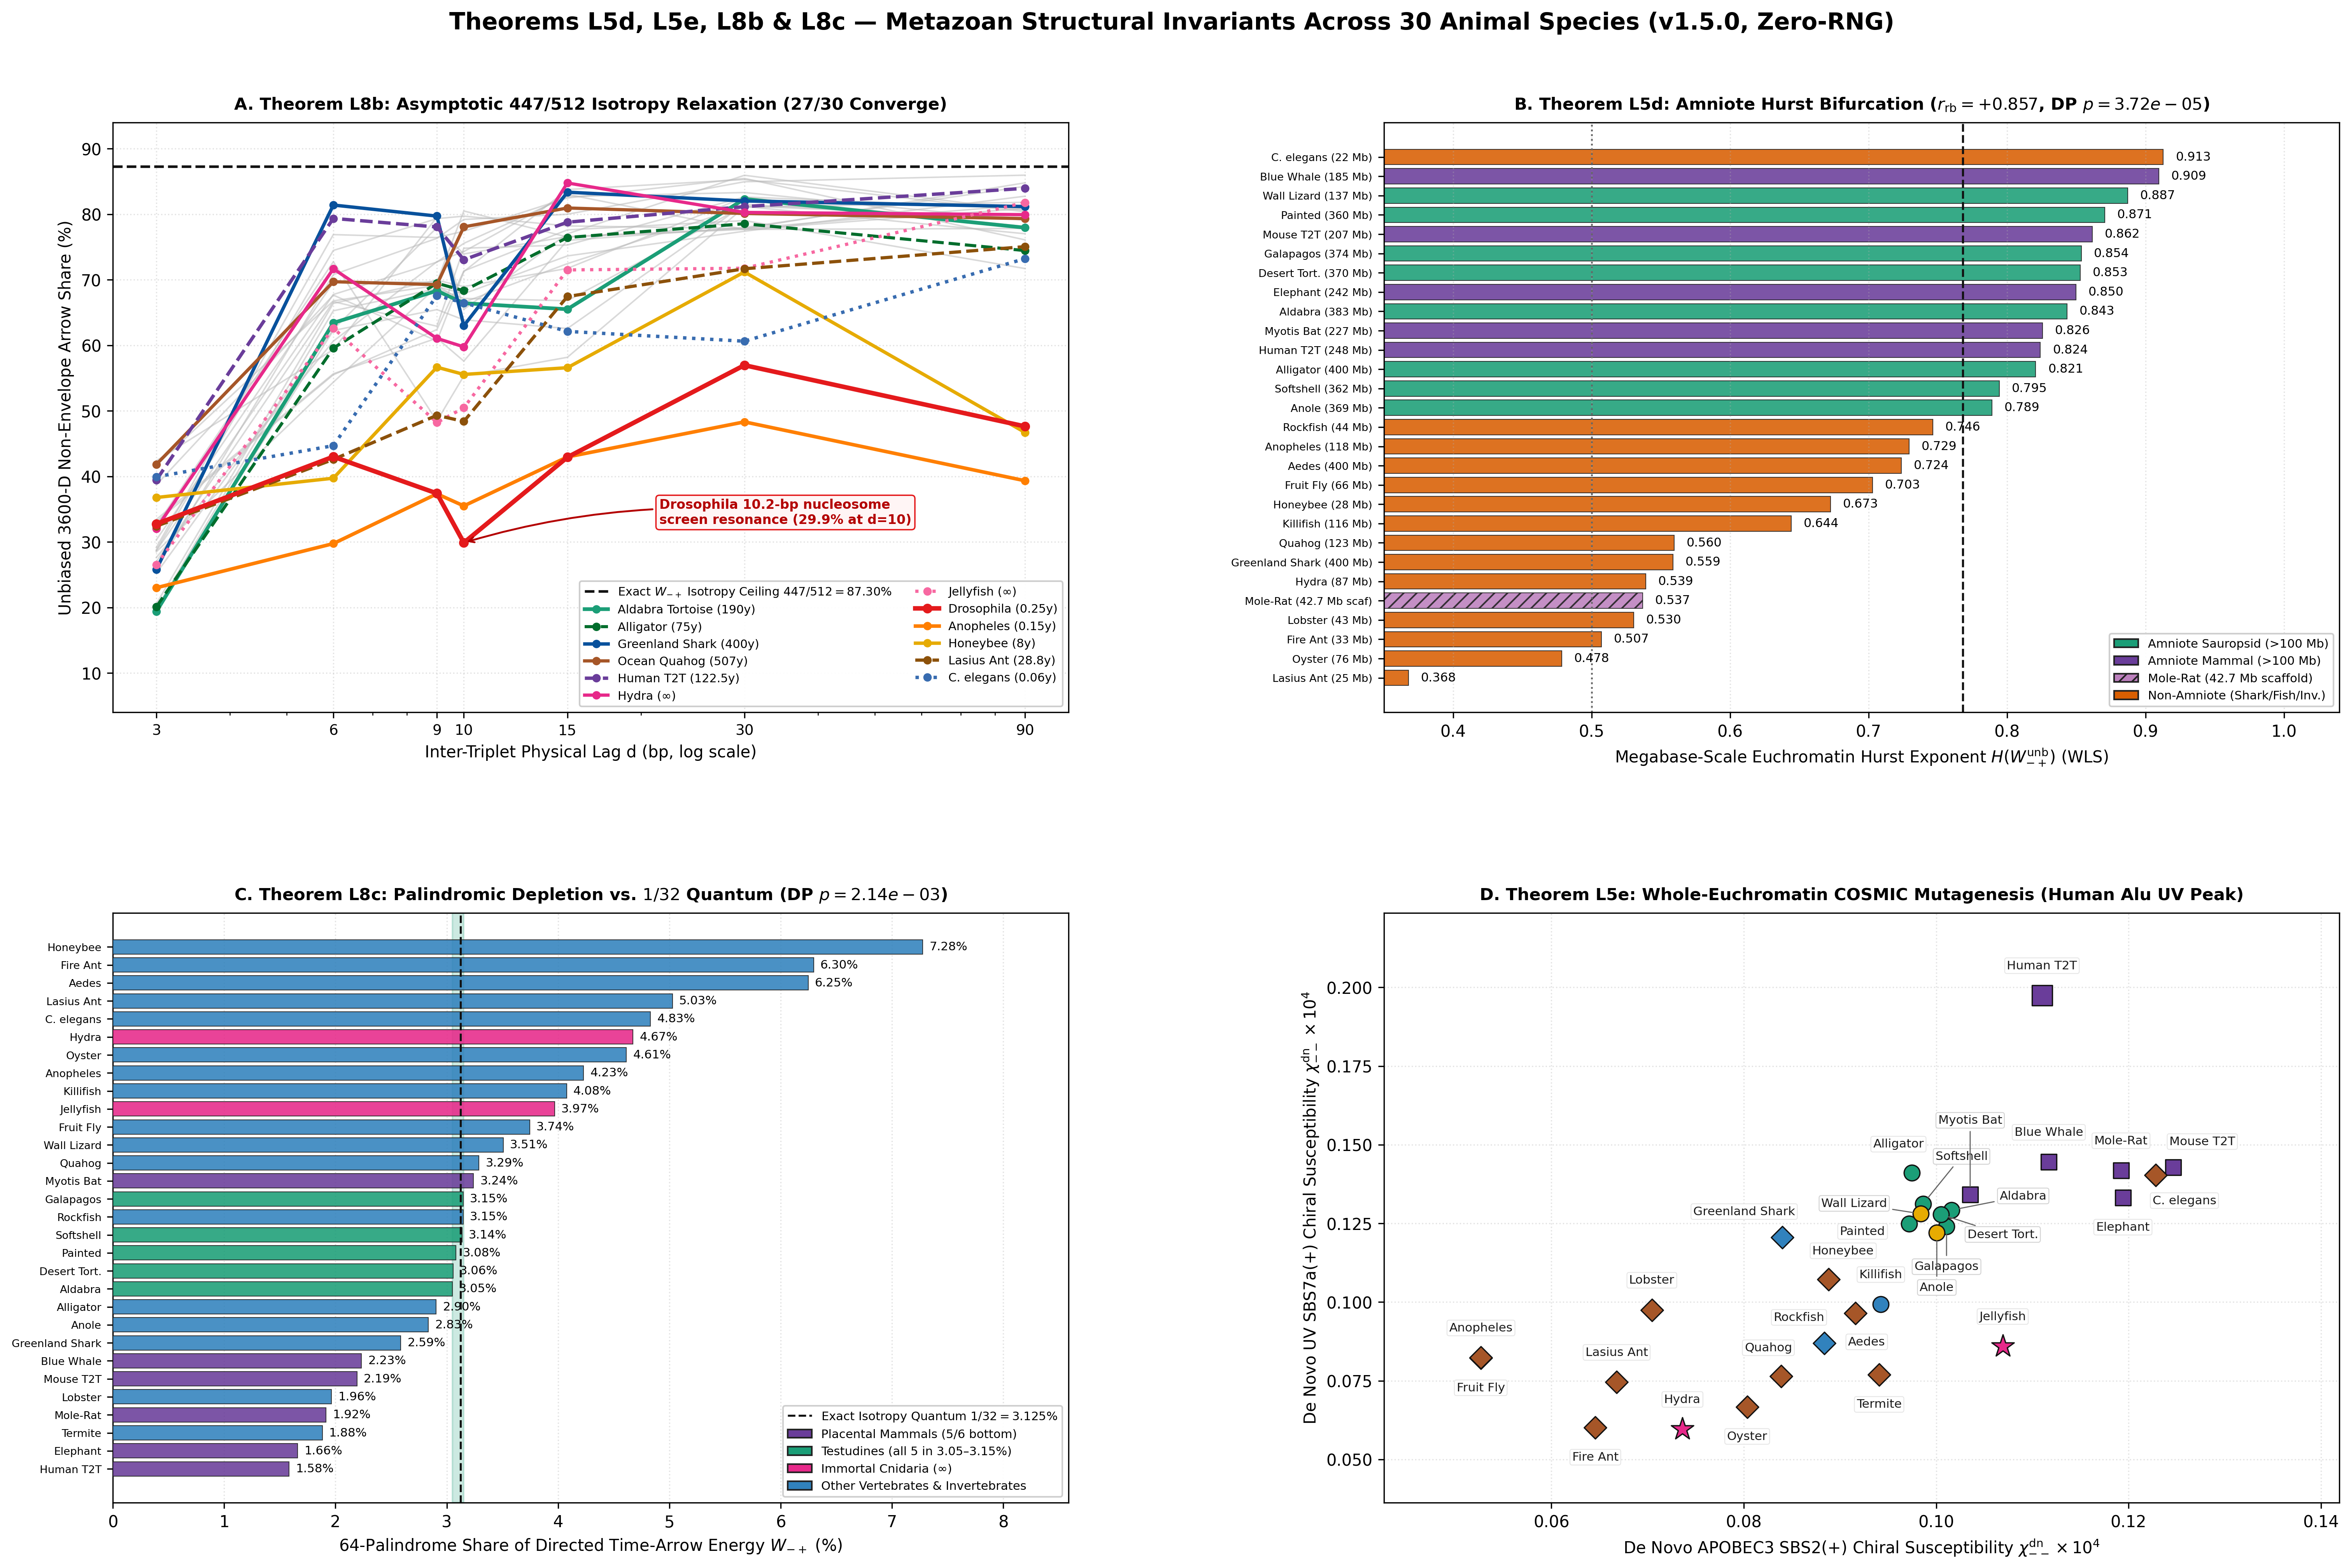
\includegraphics[width=\textwidth]{fig_L10_metazoan_invariants.png}
\caption{\textbf{Theorems~L5d, L5e, L8b, L8c \& L8g --- Four Metazoan Structural Invariants Across 30 Animal Species.}
(A) Asymptotic relaxation of unbiased $3600\text{-D}$ non-envelope share across lags $d=3\text{--}90\text{ bp}$ toward the exact $W_{-+}$ isotropy ceiling $447/512 = 87.30\%$ in $27/30$ species, contrasted with the compact-Diptera nucleosome screen lock in \textit{Drosophila} ($29.9\%$ at $d=10$) and \textit{Anopheles} ($48.3\%$ at $d=30$).
(B) Megabase-scale Hurst bifurcation $H(W_{-+}^{\mathrm{unb}})$ separating all $13/13$ full-chromosome amniotes ($0.789\text{--}0.909$) from $13/14$ non-amniotes ($0.368\text{--}0.746$; exact DP $p=3.72\times 10^{-5}$), with holocentric \textit{C.\ elegans} chrV ($0.913$) as the sole non-amniote exception.
(C) Palindromic $W_{-+}$ energy share relative to the exact isotropy quantum $1/32 = 3.125\%$ (dashed line): placental mammalian depletion ($5/6$ bottom, DP $p=2.14\times 10^{-3}$), tight Testudines crystal band ($3.05\text{--}3.15\%$, green shade), and Hymenopteran/\textit{Aedes} hyper-palindromes ($5.03\text{--}7.28\%$).
(D) Whole-euchromatin COSMIC de novo chiral susceptibility (\texttt{SBS2} APOBEC3 vs.\ \texttt{SBS7a} UV), highlighting the isolated human \textit{Alu}-driven UV peak ($\chi_{--}^{\mathrm{dn}} = 0.1975\times 10^{-4}$).}
\label{fig:L10}
\end{figure}

% =====================================================================
\section{Discussion: Five Evolutionary Genomic Strategies Across 30 Metazoans}
% =====================================================================
Our falsification-driven expansion from giant tortoises to 30 animal species resolves why naive cross-phylum longevity correlations fail while clade-resolved algebraic structure is extraordinarily sharp:
\begin{enumerate}
  \item \textbf{Archosaurian Structural Stasis (Giant Tortoises \& Alligator):} Long-lived Cryptodira turtles ($42\text{--}190\text{ yr}$) and \textit{Alligator mississippiensis} ($75\text{ yr}$) maintain ultra-quiet, low-volatility euchromatin ($I_{\mathrm{nonbr}} = 0.0081\text{--}0.0108$, $3600\text{-D} = 19.4\text{--}20.6\%$, Beyond-M2 $= 26.1\text{--}29.8\%$) that has barely drifted over $255\text{ Myr}$ ($0.0075\text{--}0.0431 / 100\text{ Myr}$).
  \item \textbf{Active High-Turnover Mammalian Longevity (Human, Blue Whale, Elephant, Bat, Mole-Rat):} Placental mammals tolerate $2\text{--}3\times$ higher euchromatin repeat memory ($I_{\mathrm{nonbr}} = 0.0133\text{--}0.0262$) and rapid $100\text{-Myr}$ structural remodeling ($0.213\text{--}0.450$), relying instead on active cellular tumor suppression (Peto's paradox mechanisms, high-molecular-mass hyaluronan, expanded \textit{TP53} networks) rather than static genomic silence.
  \item \textbf{Cold-Water, Bivalve, and Crustacean Extremes (Greenland Shark, Rockfish, Ocean Quahog, American Lobster):} The $400\text{-yr}$ Greenland shark ($43.7\%$ interspersed repeat blocks, $R_{\mathrm{mem}}=0.525$) and $100\text{-yr}$ American lobster ($I_{\mathrm{nonbr}}=0.0452$, Beyond-M2 $=121.8\%$) prove that extreme longevity is compatible with dense repeat texture, while $507\text{-yr}$ \textit{Arctica islandica} achieves low $I_{\mathrm{nonbr}}=0.0105$ yet high $3600\text{-D}=41.8\%$ within a slowly drifting bivalve architecture ($0.0650 / 100\text{ Myr}$).
  \item \textbf{Bipolar Biological Immortality and Refutation of the CpG Trap:} \textit{Turritopsis dohrnii} (cyclic transdifferentiation) remains the quietest genome in our 30-species atlas ($I_{\mathrm{nonbr}}=0.0060$, Beyond-M2 $=20.0\%$), whereas \textit{Hydra vulgaris} (continuous stem-cell turnover) sits at the opposite repeat-rich pole ($I_{\mathrm{nonbr}}=0.0332$, $R_{\mathrm{mem}}=0.573$). In raw $W_{-+}$, the two immortal cnidarians appear deceptively similar ($\cos_{W_{-+}} = +0.7974$) owing to shared AT-richness, but subtracting the stationary Markov-2 null collapses their alignment by $-0.4557$ to $\cos_{\mathrm{Beyond\text{-}M2}} = +0.3417$, while \textit{Hydra} retains a unique $3.13\times$ excess of raw 6-bp palindromes ($p_{\mathrm{pal}} = 4.89\%$ vs.\ $1/64 = 1.5625\%$ uniform, and $1.43\text{--}3.11\%$ across all other $29$ species). Short-lived Diptera ($\mathrm{CpG}$ O/E $=0.925\text{--}1.073$) and eusocial Hymenoptera ($\mathrm{CpG}$ O/E $=1.463\text{--}1.682$) decisively eliminate unmethylated $\mathrm{CpG}$ retention as a signature of immortality.
  \item \textbf{Ecdysozoa Structural Divergence (Compact Diptera, Eusocial Insects, and Holocentric Nematodes):} Within Ecdysozoa, compact nucleosome-phased Diptera (\textit{Drosophila}, \textit{Anopheles}) lock $W_{-+}$ energy inside the $130\text{-D}$ screen at $d=10\text{--}90\text{ bp}$, whereas transposable-element expansion in \textit{Aedes aegypti} releases the screen lock and drives the fastest $100\text{-Myr}$ toric drift in the atlas ($0.4881$). Independently evolved eusocial queens split across two opposite methylation architectures---hyper-CpG, hyper-palindromic Hymenoptera (\textit{Apis}, \textit{Lasius}, \textit{Solenopsis}) versus methylated, low-palindrome Blattodea (\textit{Zootermopsis})---while \textit{C.\ elegans} occupies a holocentric, poly-AT orthogonal island.
\end{enumerate}

% =====================================================================
\section{Limitations, Falsifiability, and Open-Science Reproducibility}
% =====================================================================
Three limitations merit explicit note: (i) the three giant $>400\text{ Mb}$ chromosomes (\textit{S.\ microcephalus}, \textit{A.\ mississippiensis}, \textit{A.\ aegypti}) were audited on their deterministic $400\text{ Mb}$ prefixes rather than full $465\text{--}487\text{ Mb}$ lengths, though split-half cosines $>0.984$ confirm spatial stationarity within the audited prefix; (ii) \textit{T.\ dohrnii} and \textit{Z.\ nevadensis} currently lack chromosome-level T2T assemblies and were audited via exact $100\text{-bp}$ $N$-barrier WGS pools ($40.0\text{--}40.4\text{ Mb}$); and (iii) single-chromosome audits should next be extended to complete multi-chromosome karyotypes (including avian and sauropsid microchromosomes) and broader phylogenetic sampling (birds, crocodilians, and holocentric insects such as Lepidoptera) enabling formal phylogenetic generalized least squares (PGLS).

All numbers, tables, checkpoints (\texttt{chr\_audit\_cache}, \texttt{gene\_cache}), and 300-DPI figures in this manuscript are archived at \href{https://github.com/Dr-Logvinovich/longevity-codon-torus}{\nolinkurl{github.com/Dr-Logvinovich/longevity-codon-torus}} and are reproduced with zero randomness via \href{https://github.com/Dr-Logvinovich/longevity-codon-torus/blob/main/tortoise_longevity_torus_v1_0.py}{\nolinkurl{tortoise_longevity_torus_v1_0.py}} (Engine \texttt{v1.5.0}):
{\small
\begin{verbatim}
git clone https://github.com/Dr-Logvinovich/longevity-codon-torus.git
cd longevity-codon-torus
python3 tortoise_longevity_torus_v1_0.py --self-test
python3 tortoise_longevity_torus_v1_0.py --discover-extremes
python3 tortoise_longevity_torus_v1_0.py --extremes-audit --deep-analysis --out-dir results_tortoise_v1_5
pdflatex -interaction=nonstopmode longevity_torus_v1_6.tex
\end{verbatim}
}

\section*{Acknowledgements}
We thank Christophe Chauprade (Paris) for suggesting this research on giant tortoise and extreme-longevity genomes, and Robert Friedman, MD (USA) and James Occhialini, PhD (USA) for stimulating discussions.

\appendix
\section{Complete 30-Species Top-5 Directed 6-Mer Orbit Atlas and 64/64 Self-Test Certificate}
\label{app:motifs}
Table~\ref{tab:top5_motifs} lists the five highest-flux $V_4$-canonical directed 6-mer orbits in euchromatin $W_{-+}$ across all 30 species, ranked by single-entry flux amplitude $|W_{-+}(u,v)|$ (because palindromic orbits $(u, r(u))$ have $V_4$-multiplicity $2$ rather than $4$, their total orbit energy share is half that of a non-palindromic orbit of equal entry amplitude). Whereas 28 species are dominated by AT-rich poly-tract orbits (\texttt{TTT-AAA}, \texttt{TTT-TAA}, \texttt{AAA-ATT}, \texttt{AAT-TTT}), \textit{Homo sapiens} T2T stands completely alone with five GC-rich \textit{Alu}-characteristic purine/pyrimidine orbits (\texttt{GGG-AGG}\slash\texttt{CCT-CCC}, \texttt{GCC-TCC}\slash\texttt{GGA-GGC}, \texttt{TCC-CAG}, \texttt{CCC-AGC}, \texttt{CCC-AGG}, whose reverse-complement mirrors carry the pyrimidine \texttt{SBS7a} substrates), directly explaining its elevated whole-euchromatin \texttt{SBS7a} UV susceptibility (Theorem~\ref{thm:L5cd}), while \textit{Homarus americanus} is the sole invertebrate exhibiting \texttt{GGG-AGG} ($2.6\%$, \#2) and \texttt{GGA-GGG} ($1.6\%$, \#4).

\begin{table}[H]
\centering
{\renewcommand{\arraystretch}{0.88}
\caption{\textbf{Top-5 Dominant Directed 6-Mer Orbits in Euchromatin $W_{-+}$ Across All 30 Animal Species (Flux Share \%).}}
\label{tab:top5_motifs}
\resizebox{\textwidth}{!}{%
\begin{tabular}{llllll}
\toprule
\textbf{Species} & \textbf{Top-1} & \textbf{Top-2} & \textbf{Top-3} & \textbf{Top-4} & \textbf{Top-5} \\
\midrule
\textbf{Immortal Jellyfish} & \texttt{AAA-ATT} (9.4\%) & \texttt{ATT-TTT} (5.8\%) & \texttt{AAC-ATT} (3.3\%) & \texttt{TTT-TCA} (3.0\%) & \texttt{AAA-TTT} (1.4\%) \\
\textbf{Hydra Immortal} & \texttt{TTT-TAA} (13.7\%) & \texttt{TTT-TTA} (9.0\%) & \texttt{AAA-AAT} (8.5\%) & \texttt{AAA-ATT} (6.8\%) & \texttt{AAT-ATT} (2.5\%) \\
\textbf{Ocean Quahog} & \texttt{ATA-TTT} (5.0\%) & \texttt{CAA-AAT} (4.9\%) & \texttt{AAT-ATT} (1.9\%) & \texttt{TAA-AAT} (3.6\%) & \texttt{AAC-ATT} (3.3\%) \\
\textbf{Greenland Shark} & \texttt{TTT-TAA} (1.7\%) & \texttt{TTT-AAA} (0.8\%) & \texttt{TGC-AGT} (1.3\%) & \texttt{AGA-AAT} (1.1\%) & \texttt{CAT-TTT} (1.0\%) \\
\textbf{Rougheye Rockfish} & \texttt{TTT-AAA} (2.1\%) & \texttt{TGT-TTT} (1.9\%) & \texttt{GTT-TTC} (1.8\%) & \texttt{TTT-TAA} (1.4\%) & \texttt{TTC-AGA} (1.4\%) \\
\textbf{Aldabra Tortoise} & \texttt{TTT-AAA} (1.1\%) & \texttt{TTT-TAA} (1.9\%) & \texttt{GTT-TTC} (1.4\%) & \texttt{ATT-TCA} (1.1\%) & \texttt{GGC-AGC} (1.0\%) \\
\textbf{Galapagos Tortoise} & \texttt{TTT-AAA} (1.2\%) & \texttt{TTT-TAA} (1.9\%) & \texttt{GAA-AAC} (1.4\%) & \texttt{ATT-TCA} (1.2\%) & \texttt{GCT-GCC} (1.0\%) \\
\textbf{Human T2T} & \texttt{GGG-AGG} (2.5\%) & \texttt{GCC-TCC} (2.1\%) & \texttt{TCC-CAG} (2.0\%) & \texttt{CCC-AGC} (1.6\%) & \texttt{CCC-AGG} (1.5\%) \\
\textbf{Blue Whale} & \texttt{TTT-TAA} (2.2\%) & \texttt{ATT-TCT} (1.5\%) & \texttt{GTT-TTC} (1.4\%) & \texttt{GGC-TTC} (1.1\%) & \texttt{TTT-AAA} (0.5\%) \\
\textbf{American Lobster} & \texttt{ACT-GTA} (3.6\%) & \texttt{GGG-AGG} (2.6\%) & \texttt{ACA-GTA} (2.1\%) & \texttt{GGA-GGG} (1.6\%) & \texttt{TTA-TTT} (1.5\%) \\
\textbf{Desert Tortoise} & \texttt{TTT-AAA} (1.1\%) & \texttt{TTA-AAA} (1.9\%) & \texttt{GTT-TTC} (1.4\%) & \texttt{ATT-TCA} (1.1\%) & \texttt{GGC-AGC} (0.9\%) \\
\textbf{American Alligator} & \texttt{GGC-AGC} (1.7\%) & \texttt{TTT-AAA} (0.8\%) & \texttt{GGC-TGC} (1.5\%) & \texttt{GTT-TTC} (1.2\%) & \texttt{GCC-TGC} (1.1\%) \\
\textbf{African Elephant} & \texttt{GAA-AAC} (2.2\%) & \texttt{AGA-AAT} (1.5\%) & \texttt{GGA-AAC} (1.4\%) & \texttt{TTT-TAA} (1.3\%) & \texttt{AAT-TTT} (1.1\%) \\
\textbf{Painted Turtle} & \texttt{TTT-AAA} (1.2\%) & \texttt{TTT-TAA} (2.0\%) & \texttt{GAA-AAC} (1.4\%) & \texttt{ATT-TCA} (1.1\%) & \texttt{GCA-GCC} (1.0\%) \\
\textbf{Naked Mole Rat} & \texttt{ATT-TCT} (2.0\%) & \texttt{GTT-TTC} (1.9\%) & \texttt{TTA-AAA} (1.6\%) & \texttt{TAA-AAT} (1.3\%) & \texttt{TGA-AAT} (1.1\%) \\
\textbf{Greater Mouse Eared Bat} & \texttt{TTT-TAA} (3.1\%) & \texttt{TTT-AAA} (1.1\%) & \texttt{ATA-TTT} (1.9\%) & \texttt{GAA-AAC} (1.6\%) & \texttt{TAA-AAT} (1.3\%) \\
\textbf{Black Garden Ant} & \texttt{ATA-TTT} (4.8\%) & \texttt{AAA-ATT} (4.6\%) & \texttt{ATT-TTT} (3.6\%) & \texttt{GAA-AAT} (2.6\%) & \texttt{AAA-TTT} (1.1\%) \\
\textbf{Softshell Turtle} & \texttt{TTT-AAA} (1.9\%) & \texttt{ATT-TCA} (1.5\%) & \texttt{TTA-AAA} (1.4\%) & \texttt{ATT-TTG} (1.3\%) & \texttt{GTT-TTC} (1.2\%) \\
\textbf{Pacific Oyster} & \texttt{AAA-AAT} (7.2\%) & \texttt{TTA-AAA} (7.0\%) & \texttt{AAA-TAT} (4.5\%) & \texttt{AAT-ATT} (2.0\%) & \texttt{AAT-TTT} (4.0\%) \\
\textbf{Dampwood Termite} & \texttt{AGA-AAT} (4.0\%) & \texttt{TTT-CTT} (3.2\%) & \texttt{AAA-TAT} (2.8\%) & \texttt{TGA-AAT} (2.6\%) & \texttt{CAA-AAT} (2.4\%) \\
\textbf{Wall Lizard} & \texttt{TTT-AAA} (1.6\%) & \texttt{TTT-TAA} (2.7\%) & \texttt{ATT-TCT} (1.3\%) & \texttt{GAA-AAC} (1.2\%) & \texttt{GAA-AGC} (1.1\%) \\
\textbf{Honeybee} & \texttt{AAA-ATT} (7.3\%) & \texttt{AAA-TAT} (5.5\%) & \texttt{AAA-TTT} (2.0\%) & \texttt{ATT-TTT} (4.0\%) & \texttt{ATC-GAT} (1.2\%) \\
\textbf{Green Anole} & \texttt{TTT-AAA} (1.3\%) & \texttt{TTT-TAA} (2.2\%) & \texttt{GAA-AAC} (2.1\%) & \texttt{AAC-ATT} (1.9\%) & \texttt{ATT-TCT} (1.6\%) \\
\textbf{Fire Ant} & \texttt{AAA-ATT} (10.2\%) & \texttt{ATT-TTT} (7.3\%) & \texttt{ATA-TTT} (5.6\%) & \texttt{AAT-ATT} (2.7\%) & \texttt{AAA-TTT} (1.5\%) \\
\textbf{House Mouse} & \texttt{TTT-CTT} (2.2\%) & \texttt{TTC-TTT} (2.1\%) & \texttt{GTT-TTC} (1.4\%) & \texttt{TTT-GTT} (1.3\%) & \texttt{TTT-TAA} (1.3\%) \\
\textbf{Turquoise Killifish} & \texttt{TTT-AAA} (2.8\%) & \texttt{TTT-TAA} (3.4\%) & \texttt{GAA-AAC} (1.9\%) & \texttt{AAC-ATT} (1.6\%) & \texttt{TAT-TTA} (1.4\%) \\
\textbf{Fruit Fly} & \texttt{TGG-CCA} (2.0\%) & \texttt{AAA-TAT} (3.8\%) & \texttt{AAA-AGT} (2.2\%) & \texttt{AAA-ATG} (2.0\%) & \texttt{ATT-TAT} (1.7\%) \\
\textbf{Malaria Mosquito} & \texttt{AAC-ATT} (1.7\%) & \texttt{ATC-GAT} (0.8\%) & \texttt{CGA-TCG} (0.8\%) & \texttt{ATT-TAT} (1.5\%) & \texttt{GTT-TTG} (1.4\%) \\
\textbf{Yellow Fever Mosquito} & \texttt{AAT-TTT} (11.0\%) & \texttt{AAA-AAT} (10.2\%) & \texttt{AAA-TTT} (3.9\%) & \texttt{TTT-TTC} (4.2\%) & \texttt{AAT-ATT} (1.7\%) \\
\textbf{Roundworm (\textit{C.\ elegans})} & \texttt{AAT-TTT} (19.0\%) & \texttt{ATT-TTT} (16.6\%) & \texttt{AAA-TTT} (4.0\%) & \texttt{GAA-AAA} (6.3\%) & \texttt{TTT-TTG} (4.1\%) \\
\bottomrule
\end{tabular}}}
\end{table}

\subsection{Zero-RNG Algebraic Verification Certificate (64/64 Checks Passed)}
\label{app:selftest}
Every execution of \href{https://github.com/Dr-Logvinovich/longevity-codon-torus/blob/main/tortoise_longevity_torus_v1_0.py}{\nolinkurl{tortoise_longevity_torus_v1_0.py}} (v1.5.0, SHA-256 \texttt{a509e148\allowbreak a8c0608b\allowbreak e7d3c81d\allowbreak 74168b3e\allowbreak 3ac318f3\allowbreak 0854a26c\allowbreak 38e104c9\allowbreak 7bb545db}) enforces static AST prohibition of random modules and passes \textbf{64/64 closed-form algebraic self-tests} with machine-precision residuals:
\begin{itemize}
  \item \textbf{Klein $V_4$ equivariance \& PR2 exactness (\#01--\#05):} revcomp error $= 0.0$, exact PR2 $W_{--} = 0.0$, $E_{\mathrm{het}}$ annihilation $= 1.93 \times 10^{-36}$, screen KL chain error $= 4.44 \times 10^{-16}$.
  \item \textbf{Screen envelope $\Pi_{\mathrm{env}}$ \& U-stat Pythagorean split (\#06--\#07):} $[g, \Pi_{\mathrm{env}}]$ commutator error $= 2.22 \times 10^{-16}$, unbiased $496+3600$ Pythagorean error $= 4.34 \times 10^{-19}$.
  \item \textbf{Null tower \& COSMIC mutagenesis (\#11--\#21):} Markov-1/2 non-bridge residuals $< 10^{-16}$, SBS1 de novo chirality $= 3.27 \times 10^{-33}$, parallelogram error $= 0.0$, isolated CpG angle error $= 0.0$, universal $705/256$ barrier error $= 0.0$, 64-palindrome chiral blindness $= 0.0$.
  \item \textbf{Exact DP statistics, WGS $N$-barriers \& FWL controls (\#22--\#56):} Mann--Whitney DP error $= 0.0$, paired sign-test error $= 0.0$, multi-FASTA / FTP-WGS $N$-barrier cross-boundary error $= 0.0 / 0.0$, zero-overlap AABB label audit passed.
  \item \textbf{Metazoan structural invariants \& native Figure~5 checks (\#57--\#60):} exact $447/512$ isotropy fraction verified, Amniote Hurst DP error $= 0.0$, Mammalian palindromic DP check passed, native \texttt{fig\_L10} renderer verified.
  \item \textbf{Palindromic $1/32$ quantum, radial--angular identity \& exact DP separations (\#61--\#64):} exact rank $\dim(\mathcal{P}_{\mathrm{pal}}\cap W_{-+}) = 32$ ($32/1024 = 1/32$) verified, radial--angular Pythagorean residual $= 2.22 \times 10^{-16}$, exact complete-separation DP checks passed ($0.0$ error).
\end{itemize}

\begin{thebibliography}{99}
\bibitem{Perez1991} J.-C.~Perez, ``Chaos DNA and neuro-computers: A golden link,'' \textit{Speculations in Science and Technology} \textbf{14}(4), 336--346 (1991).
\bibitem{Perez1997} J.-C.~Perez, \textit{L'ADN d\'ecrypt\'e: la d\'ecouverte des preuves math\'ematiques de l'intelligence du vivant}, \'Editions Marco Pietteur (Collection R\'esurgence), Li\`ege (1997).
\bibitem{Perez2009} J.-C.~Perez, \textit{Codex Biogenesis: Les 13 codes de l'ADN}, \'Editions Marco Pietteur (Collection R\'esurgence), Li\`ege (2009).
\bibitem{Perez2010} J.-C.~Perez, ``Codon populations in single-stranded whole human genome DNA are fractal and fine-tuned by the Golden Ratio 1.618,'' \textit{Interdisciplinary Sciences: Computational Life Sciences} \textbf{2}(3), 228--240 (2010), doi:\href{https://doi.org/10.1007/s12539-010-0022-0}{10.1007/s12539-010-0022-0}; Erratum: \textbf{2}(4), 373 (2010); PMID:~20658335.
\bibitem{Perez2015} J.-C.~Perez, ``Deciphering Hidden DNA Meta-Codes --- The Great Unification \& Master Code of Biology,'' \textit{Journal of Glycomics \& Lipidomics} \textbf{5}(2), 131 (2015).
\bibitem{Perez2017} J.-C.~Perez, ``Sapiens mitochondrial DNA genome circular long range numerical meta structures are highly correlated with cancers and age-associated diseases,'' \textit{Journal of Cancer Therapy} \textbf{8}(5), 512--538 (2017).
\bibitem{Perez2018} J.-C.~Perez, ``Six fractal codes of biological life: Perspectives in exobiology, cancers and artificial intelligence,'' \textit{Biomedical Journal of Scientific \& Technical Research} \textbf{9}(2), 6954--6969 (2018).
\bibitem{Perez2021} J.-C.~Perez, ``Creation of synthetic genomes: Numerical resonances and Master Code audits,'' \textit{International Journal of Research --- Granthaalayah} \textbf{9}(6), 1--28 (2021).
\bibitem{PerezMontagnier2021} J.-C.~Perez and L.~Montagnier, ``Six fractal codes of life from bioatoms atomic mass to chromosomes numerical standing waves: Three breakthroughs in astrobiology, cancers and artificial intelligence,'' \textit{International Journal of Research --- Granthaalayah} \textbf{9}(9), 133--191 (2021), doi:\href{https://doi.org/10.29121/granthaalayah.v9.i9.2021.4191}{10.29121/granthaalayah.v9.i9.2021.4191}.
\bibitem{Perez2022} J.-C.~Perez, ``Epigenetics theoretical limits of synthetic genomes,'' \textit{Global Journal of Science Frontier Research G} \textbf{22}(2), 35--47 (2022).
\bibitem{LogvinovichPerez2026a} V.~Logvinovich and J.-C.~Perez, \textit{The Double-Stranded Codon Torus: Exact Klein $V_4$ Spectral Algebra and Zero-RNG Genomic Forensics}, Zenodo Record 23695321 (2026).
\bibitem{LogvinovichPerez2026b} V.~Logvinovich and J.-C.~Perez, \textit{The Codon Memory Spectrum on the Double-Stranded Torus: Exact Zero-RNG Null Towers, Klein Four-Group Symmetry Breaking, and the Two-Sided $16\times 16$ Dinucleotide Screen}, ResearchGate Publication 417926819 (2026).
\bibitem{Quesada2019} V.~Quesada \textit{et al.}, ``Giant tortoise genomes provide insights into longevity and age-related disease,'' \textit{Nature Ecology \& Evolution} \textbf{3}, 87--95 (2019).
\bibitem{Cilingir2022} F.~G.~\c{C}ilingir \textit{et al.}, ``Chromosome-level genome assembly for the Aldabra giant tortoise enables insights into the genetic basis of longevity,'' \textit{GigaScience} \textbf{11}, giac090 (2022).
\bibitem{Kolora2021} S.~R.~R.~Kolora \textit{et al.}, ``Origins and evolution of extreme life span in Pacific Ocean rockfishes,'' \textit{Science} \textbf{374}, 842--847 (2021).
\bibitem{PascualTorner2022} M.~Pascual-Torner \textit{et al.}, ``Comparative genomics of mortal and immortal cnidarians unveils novel keys behind rejuvenation,'' \textit{Proceedings of the National Academy of Sciences} \textbf{119}, e2118763119 (2022).
\bibitem{Kittler1986} J.~Kittler and J.~Illingworth, ``Minimum error thresholding,'' \textit{Pattern Recognition} \textbf{19}, 41--47 (1986).
\bibitem{Killick2012} R.~Killick, P.~Fearnhead, and I.~A.~Eckley, ``Optimal detection of changepoints with a linear computational cost,'' \textit{Journal of the American Statistical Association} \textbf{107}, 1590--1598 (2012).
\end{thebibliography}

\end{document}
